% Write-up of the undercast forecast at lucasehinger.github.io/weather/.
% Build:   cd files/weather/report && latexmk -pdf undercast_report.tex
% Figures: python3 scripts/build_weather_report_figures.py (from the repo root)
\documentclass[11pt]{article}
\usepackage[margin=1in]{geometry}
\usepackage[T1]{fontenc}
\usepackage{lmodern}
\usepackage{graphicx}
\usepackage{booktabs}
\usepackage{tabularx}
\usepackage{array}
\usepackage{caption}
\usepackage{subcaption}
\usepackage{amsmath}
\usepackage{xcolor}
\usepackage[section]{placeins}
\usepackage[hidelinks]{hyperref}
\usepackage[nameinlink]{cleveref}

\graphicspath{{figures/}{../examples/model_training_images/}}
\captionsetup{font=small,labelfont=bf}
\newcommand{\code}[1]{\texttt{#1}}
\newcolumntype{Y}{>{\raggedright\arraybackslash}X}

\title{Forecasting Undercasts on Mount Washington}
\author{Lucas Ehinger\\\small Massachusetts Institute of Technology\\\small\url{https://lucasehinger.github.io/weather/}}
\date{October 2026}

\begin{document}
\maketitle

\begin{abstract}
An \emph{undercast} is a cloud deck lying below a summit, leaving the summit in clear air above it.
This document describes the undercast forecast published at \url{lucasehinger.github.io/weather/}
for the 6{,}288\,ft summit of Mount Washington, New Hampshire, together with the analysis behind it.
Hand-labelled webcam images give only 22 undercast days, so labels are instead derived from the
remarks Mount Washington Observatory observers append to the hourly KMWN METAR. Five cuts on those
remarks reach precision 0.70 and recall 0.73 against the webcam labels and yield 6{,}852 undercast
hours among 253{,}317 observations from 1997--2026. A simple physics rule based on a modelled
inversion reaches only precision 0.09 at a 3\% base rate. The forecast in production is a single
gradient-boosted tree model fed by six numerical weather prediction (NWP) sources (HRRR, RAP, NAM,
GFS, ECMWF, NBM). On a held-out year with a 2.5\% base rate, it reaches ROC-AUC 0.941 and precision
0.74 one hour ahead, falling to ROC-AUC 0.764 and precision 0.08 six days ahead. The limiting factor
is the quality of the labels, not the classifier.
\end{abstract}

\tableofcontents

%======================================================================
\section{Introduction}
%======================================================================
For hikers, undercasts are a treat and are often unexpected. The project began with the assumption
that a cloud-base forecast (e.g.\ from Windy) would be enough to predict them. It is not. Undercasts
require a temperature inversion that traps cool, moist air below the summit~\cite{mwobs,gmc}, but a
modelled inversion on its own is a weak predictor (\cref{sec:physics}). Academic literature on
undercasts specifically is sparse; \cite{sd,blm,esw} are useful starting points.

The website (\cref{sec:site}) publishes an hourly undercast forecast for Mount Washington up to six
days ahead. The rest of this document covers how its training labels are built
(\cref{sec:labels}), why a physics rule fails (\cref{sec:physics}), how the machine-learning (ML)
model is built and validated (\cref{sec:ml}), and its limitations (\cref{sec:limits}).
Interactive views and per-source breakdowns from the website are collected in the appendices.

%======================================================================
\section{The website}\label{sec:site}
%======================================================================
The forecast page, \url{/weather/}, has a summit selector (Mt.\ Washington, Mt.\ Lafayette,
Mt.\ Moosilauke, Mt.\ Monadnock), a set of quick links to external forecasts for the selected summit
(\cref{app:links}), a collapsible overview of the NWP sources (\cref{tab:nwp}), and two panels:
\begin{description}
\item[Undercast forecast.] An hourly strip covering the coming forecast window. Each bar's height is
  the model's score for that hour divided by the decision threshold for that hour's forecast lead,
  with a dashed line marking the threshold. Hours at or above the line are called undercast, and the
  panel names the first undercast window. Hours already in the past are dropped. If a required NWP
  source did not publish in time, the panel says \emph{Forecast unavailable} rather than showing a
  quiet forecast. This is deliberate: a missing forecast must not read as ``no undercast''.
\item[Model performance.] A collapsible panel with the held-out-year confusion matrix of the
  production model at each forecast lead (1, 24, 48, 72, 96, 120 and 144\,h), using the same
  thresholds as the forecast (\cref{tab:final}).
\end{description}
The undercast model is trained on Mount Washington observations only (\cref{sec:labels}) and does
not transfer to the other summits. When another summit is selected, the page says the prediction is
only available for Mt.\ Washington. A GitHub Actions job refreshes the forecast every six hours.

Four supporting pages document the analysis: \emph{Model Details} (\url{/weather/details/}, the main
write-up), \emph{What the Cuts Keep and Throw Away} (\url{/weather/cuts/}, a webcam gallery of the
label cuts), \emph{Observation Viewer} (\url{/weather/observations/}, 42 METAR reports beside their
webcam frames) and \emph{What the Models Actually Show}
(\url{/weather/historical-conditions/}, the inversion analysis plus a day-by-day viewer of the
NWP profiles and the noon webcam image).

\begin{table}[ht]\centering\small
\caption{NWP sources as summarised on the forecast page and the details page. Range is the forecast
range used on the site.}\label{tab:nwp}
\begin{tabularx}{\linewidth}{l l l Y}
\toprule
Model & Range (h) & Resolution & Notes\\
\midrule
HRRR & 0--48 & 3\,km, CONUS & High-Resolution Rapid Refresh; hourly, short range; cloud fields\\
RAP  & 0--48 & 13\,km, regional & HRRR's parent model; cloud fields\\
NAM  & 0--60 & 12\,km, regional & North American Mesoscale; cloud fields\\
GFS  & 0--120 & $\sim$0.25$^\circ$, global & Long range, coarse; cloud fields\\
ECMWF & 0--144 & $\sim$0.25$^\circ$, global & IFS open data; strong dynamics but no cloud fields; 3-hourly steps\\
NBM  & 0--144 & $\sim$2.5\,km, CONUS & National Blend of Models; calibrated, surface fields only, incl.\ probabilistic ceiling and visibility\\
\bottomrule
\end{tabularx}
\end{table}

%======================================================================
\section{Labels: when was it actually undercast?}\label{sec:labels}
%======================================================================
\subsection{Webcam labels}
The Mount Washington Observatory (MWOBS) archives roughly two years of daily timelapses from two
summit webcams (the \emph{tower} and \emph{observatory} cameras). Every noon frame was labelled by
hand. That gives 589 days from 25~May~2024 to 3~January~2026, of which 22 are undercast. Labelling
was generous: partial undercasts (visible on one camera only, or a broken deck) count as undercast.
Because the timelapses fade from one day into the next, some frames blend two days. A clean frame
with a matching timestamp is used wherever one exists. Twenty-two positives is too few to train a
classifier, but enough to validate a labelling rule.

\subsection{Observer remarks}
KMWN is one of the few remaining staffed weather stations in the U.S. Every hour, observers add
free-text remarks to the automated METAR. The key remark is \code{TPS LWR} (``tops lower''), which
gives the coverage and the top height (feet above sea level) of a cloud deck below the summit. For
example:
\begin{center}\small
\code{KMWN 211559Z 06010KT 70SM SCT/// OVC070 09/M06 RMK TPS LWR SCT040 SUN DMLY VSBL BINOVC}
\end{center}
Here the visibility is 70\,SM (observers estimate it from distant landmarks; automated stations stop
at 10). \code{SCT///} is a scattered layer of unknown height, and \code{OVC070} is an overcast lid
7{,}000\,ft above the station. \code{TPS LWR SCT040} is a scattered deck topping out at 4{,}000\,ft,
2{,}288\,ft below the observer. \code{SUN DMLY VSBL} means the sun is dimly visible through the
layer above, and \code{BINOVC} means breaks in the overcast. Heights in the METAR body are above the
station; \code{TPS LWR} heights are above sea level.

\subsection{The cuts}
Using the webcam days as truth, five conditions on the remarks were chosen (\cref{tab:cuts}). An hour
is \emph{undercast} if it passes all five. It is \emph{ambiguous}, and excluded from training, if it
fails at least one but still passes every looser bound in \cref{tab:cuts}. Otherwise it is \emph{not
undercast}.

\begin{table}[ht]\centering\small
\caption{Label cuts on the KMWN remarks. Heights are relative to the 6{,}288\,ft summit.}\label{tab:cuts}
\begin{tabularx}{\linewidth}{l l l Y}
\toprule
Test & Undercast & Ambiguous & Reason\\
\midrule
\code{TPS LWR} coverage & BKN or OVC & also SCT & at least 5/8 of the sky below the summit is covered\\
Visibility & $>40$\,SM & $>25$\,SM & poor visibility means the summit is at least partly in cloud\\
Deck top below summit & $\ge500$\,ft & $\ge250$\,ft & a deck just below the summit means you are mostly in it\\
Lowest layer overhead, any cover & $\ge1{,}000$\,ft & $\ge500$\,ft & e.g.\ \code{FEW002} touches the summit and passes the ceiling test\\
Lowest BKN/OVC ceiling overhead & $\ge5{,}000$\,ft & $\ge3{,}500$\,ft & a low lid makes a cloud ``sandwich'', not an undercast\\
\bottomrule
\end{tabularx}
\end{table}

\Cref{fig:ablation} shows the cuts added one at a time, starting from ``the observer reported a deck
below the summit'' (21 undercasts caught, 92 false alarms) and ending at 16 caught and 7 false alarms.
Nearly all the recall is present at the start; the cuts mainly strip out false alarms.
\Cref{tab:dropone} drops one cut at a time. Coverage is the only real trade-off: it removes 25 false
alarms but costs four genuine undercasts, all decks the observer called SCT. Scored against all 589
webcam days, the full set of cuts has \textbf{precision 0.70 and recall 0.73}.

\begin{figure}[ht]\centering
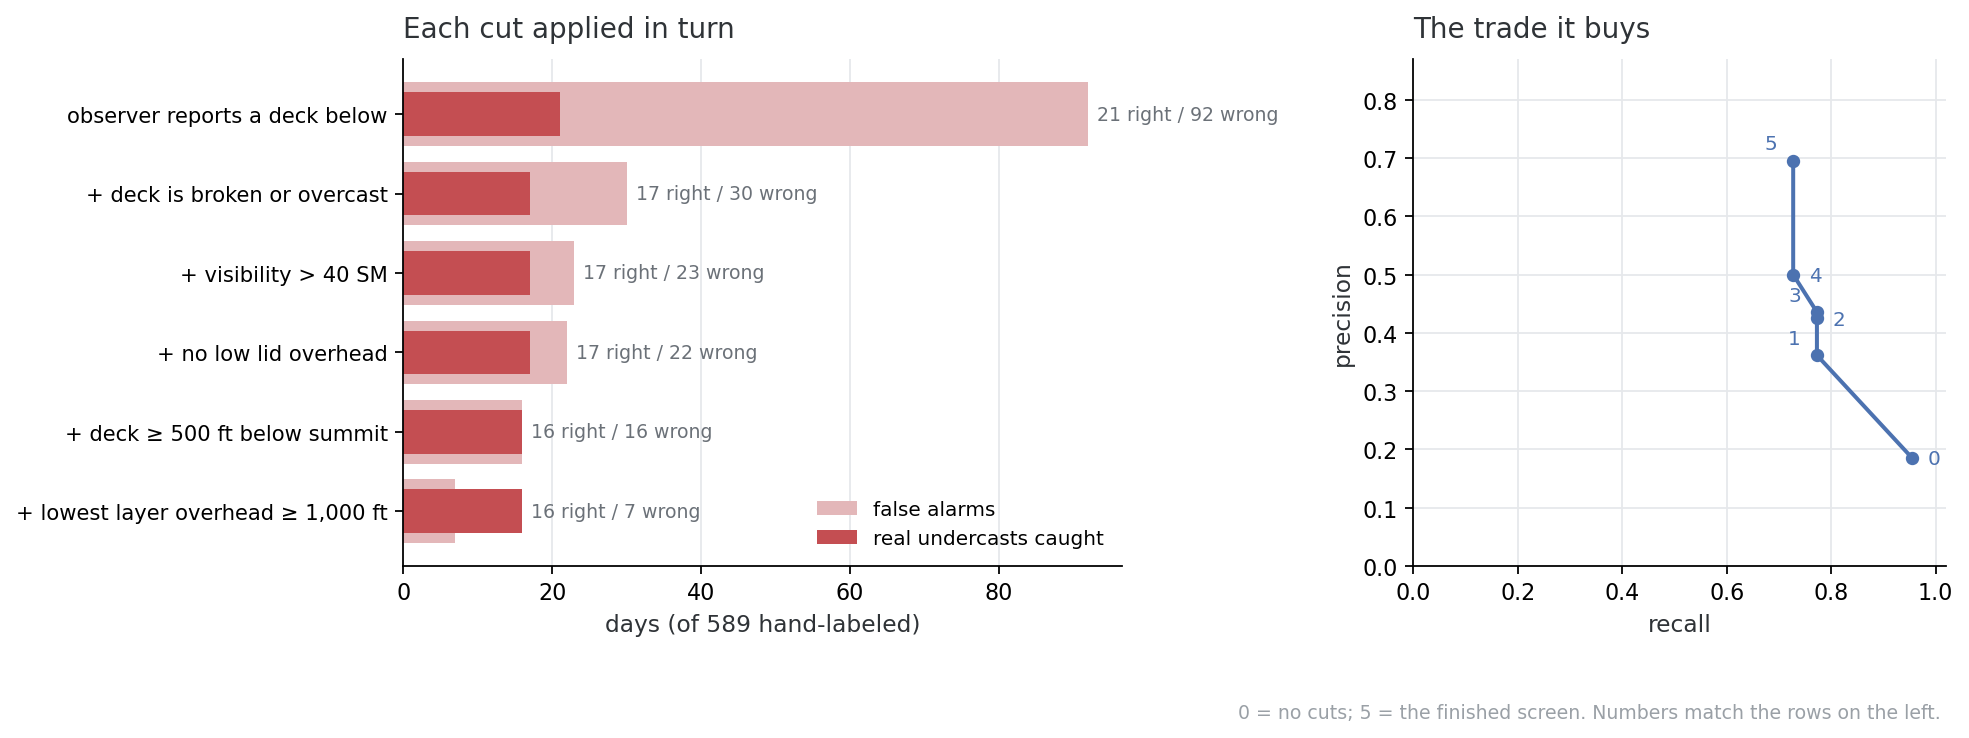
\includegraphics[width=\linewidth]{screen_cut_ablation.png}
\caption{Cuts applied cumulatively on the webcam-labelled days. Left: undercasts caught against
false alarms at each stage. Right: the same stages as precision against recall.}\label{fig:ablation}
\end{figure}

\begin{table}[ht]\centering\small
\caption{Effect of removing each cut from the full set, on the webcam days.}\label{tab:dropone}
\begin{tabular}{l r r r}
\toprule
Cut dropped & Extra false alarms & Extra undercasts caught & Precision\\
\midrule
BKN or OVC coverage & $+25$ & $+4$ & 0.38\\
Lowest layer overhead $\ge1{,}000$\,ft & $+9$ & 0 & 0.50\\
Deck $\ge500$\,ft below summit & $+3$ & 0 & 0.62\\
Visibility $>40$\,SM & $+1$ & 0 & 0.67\\
No low lid overhead & $+1$ & 0 & 0.67\\
\bottomrule
\end{tabular}
\end{table}

The cuts page shows every labelled day on which the observer reported a deck below the summit
(113 days), grouped by outcome. 23 pass every cut, 16 of them true undercasts. 29 fail only on
coverage (4 undercast). 1 fails only on visibility, 1 only on the lid, 3 only on depth and 9 only on
the lowest overhead layer, none of them undercast. 47 fail two or more cuts (1 undercast). The gallery
also shows why precision tops out near 0.70. The remark records how much of the sky a deck covers,
not how much of the horizon it fills. \code{BKN} is written the same way for an unbroken floor of
cloud and for scattered cumulus with open valleys, so no threshold on these numbers can tell the two
apart (\cref{fig:webcam}).

\begin{figure}[ht]\centering
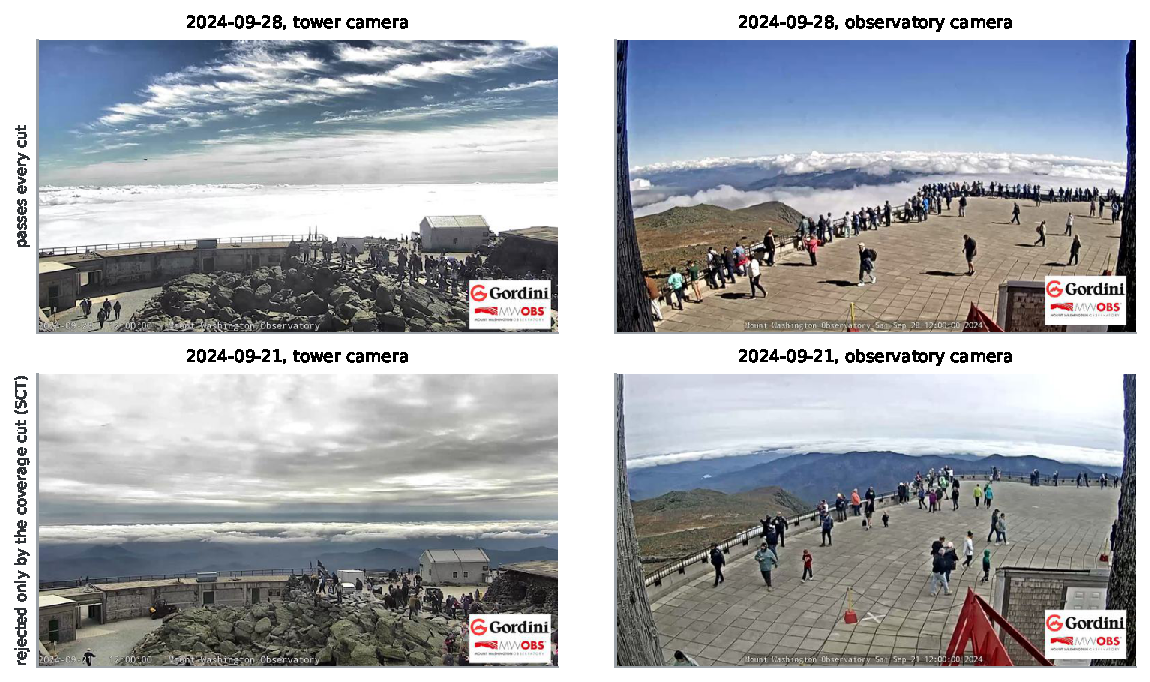
\includegraphics[width=0.85\linewidth]{webcam_examples.pdf}
\caption{Noon webcam frames. Top: a day that passes every cut. Bottom: a hand-labelled undercast
rejected only because the observer coded the deck SCT.}\label{fig:webcam}
\end{figure}

\subsection{The 29-year record}
Applied to all 253{,}317 hourly KMWN observations from 1997 to 2026, the cuts pass 6{,}852 hours as
undercast. That is over 300 times more positive examples than the webcam labels provide
(\cref{fig:scale}). The share of passing observations rises from 1.2\% in 1997 to 5.4\% in 2024
(\cref{fig:drift}). This tracks a rise in how often observers mention a deck at all, so it is most
likely a change in reporting practice, not in climate. To keep a model from learning the calendar,
every undercast observation is matched with non-undercast observations from the same year, month and
hour of day.

\begin{figure}[ht]\centering
\begin{subfigure}{0.49\linewidth}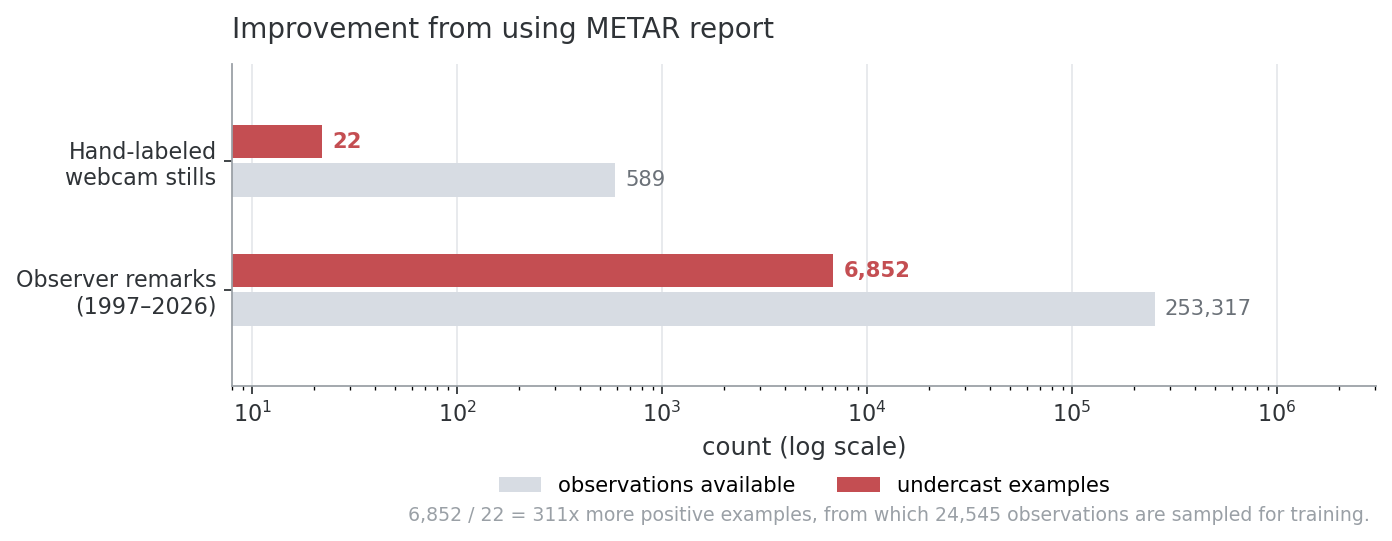
\includegraphics[width=\linewidth]{training_data_scale.png}
\caption{Labelled data from each source (log scale).}\label{fig:scale}\end{subfigure}\hfill
\begin{subfigure}{0.49\linewidth}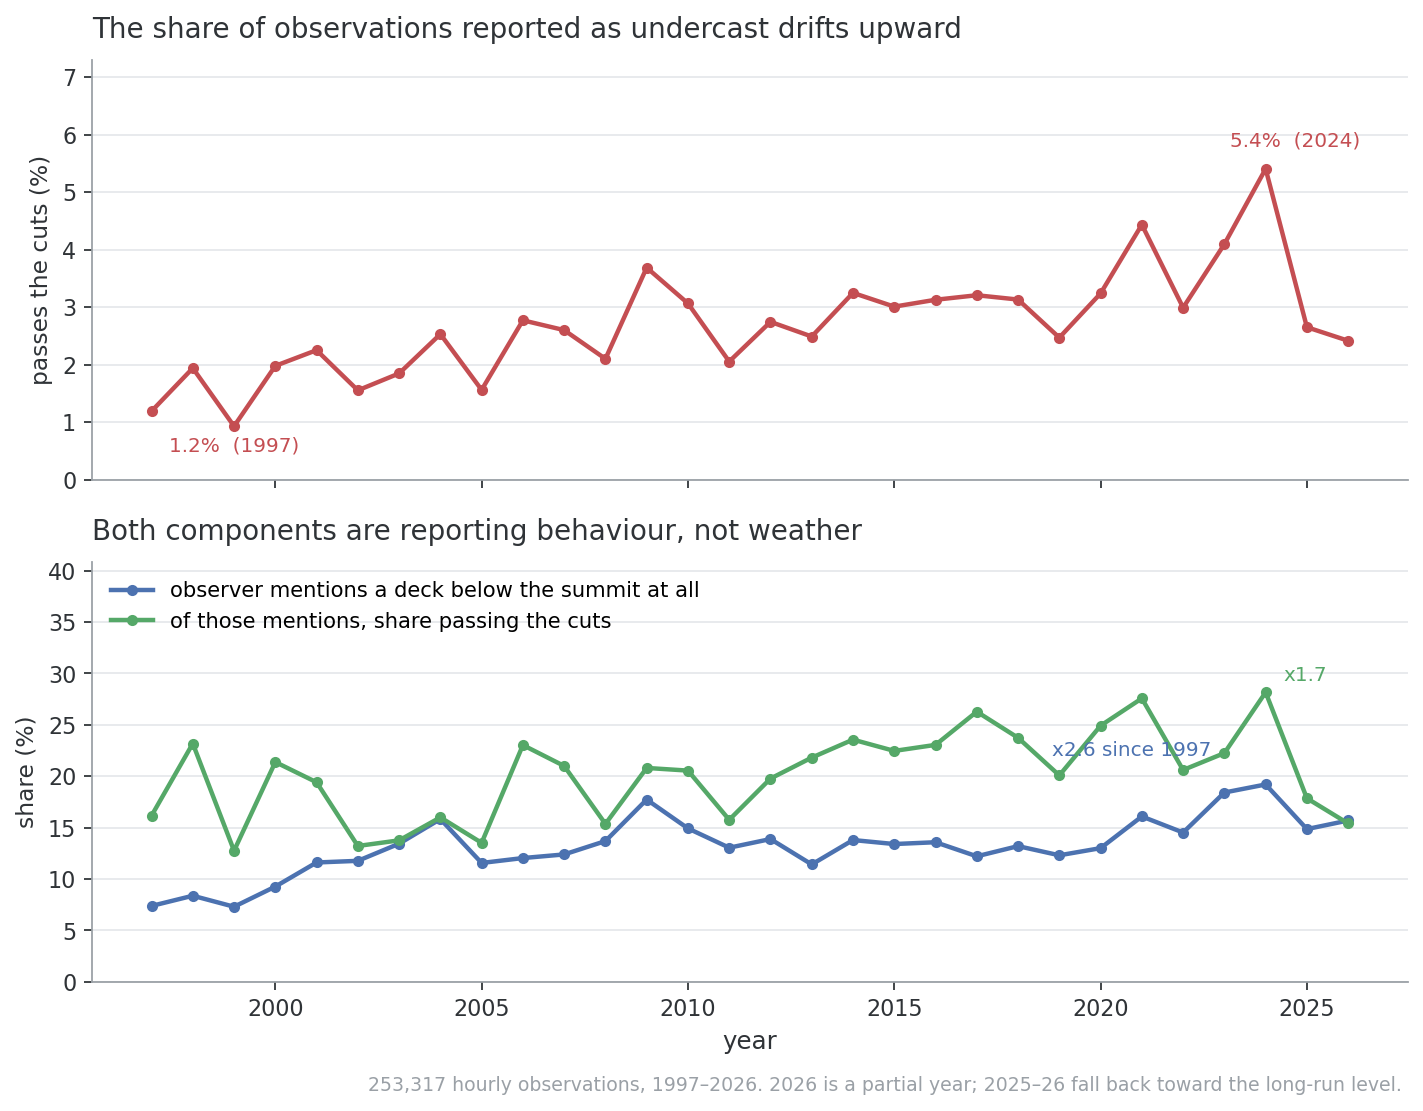
\includegraphics[width=\linewidth]{undercast_rate_drift.png}
\caption{Pass rate by year (top) and its components (bottom).}\label{fig:drift}\end{subfigure}
\caption{The remark-derived undercast record.}
\end{figure}

%======================================================================
\section{A physics-based baseline}\label{sec:physics}
%======================================================================
The first attempt used hand-written rules on the NWP output (\cref{tab:rules}), with thresholds fitted
on the training split.

\begin{table}[ht]\centering\small
\caption{Physics rules (top) and their best performance on the held-out year at a $\sim$3\% base rate
(bottom). The random baseline fires as often as HRRR's rule D.}\label{tab:rules}
\begin{tabularx}{\linewidth}{l Y}
\toprule
A: inversion & $T_{850} > T_{925}$ by more than a fitted margin: a capping inversion in the layer just below the summit\\
B: summit above deck & no modelled ceiling, or one above 1{,}917\,m\\
C & A and B\\
D & C and modelled surface visibility above a threshold\\
\bottomrule
\end{tabularx}\\[6pt]
\begin{tabular}{l l r r r}
\toprule
Source & Best rule & Precision & Recall & False alarms\\
\midrule
Random & --- & 0.03 & 0.21 & 1{,}751\\
HRRR & D & 0.09 & 0.60 & 1{,}651\\
NAM & D & 0.07 & 0.53 & 1{,}879\\
RAP & D & 0.07 & 0.48 & 1{,}743\\
GFS & C & 0.07 & 0.44 & 1{,}604\\
ECMWF & A (no ceiling field) & 0.06 & 0.68 & 1{,}975\\
\bottomrule
\end{tabular}
\end{table}

The best rule is about three times better than chance, which still makes it useless in practice. Two
rules that seemed obvious made things worse. Requiring a modelled cloud top below the summit
\emph{selects against} undercast: HRRR rows with a cloud top below 1{,}917\,m have a 9.2\% undercast
rate, compared with 16.8\% overall and 21.5\% when HRRR reports no cloud. Adding a low-cloud-fraction
term lowers the training F1 of every rule combination, from 0.41 to 0.09. Both failures come from
terrain resolution. HRRR's 3\,km grid flattens the summit cell to roughly 1{,}200\,m, so there is no
model atmosphere between its ground and the observer. Fields on pressure surfaces are less sensitive
to this.

\Cref{fig:inversion} compares the distributions directly for 24{,}315 HRRR near-analysis hours
(3{,}597 undercast). The 850--925\,mb temperature difference is the single most informative quantity
in the dataset. Undercast hours are about 1.5\,K more stable in that layer, yet 36\% of them fall on
the ``no inversion'' side of the best threshold. Every panel shows a real shift, and none shows a
clean split. That is why this is a machine-learning problem.

\begin{figure}[ht]\centering
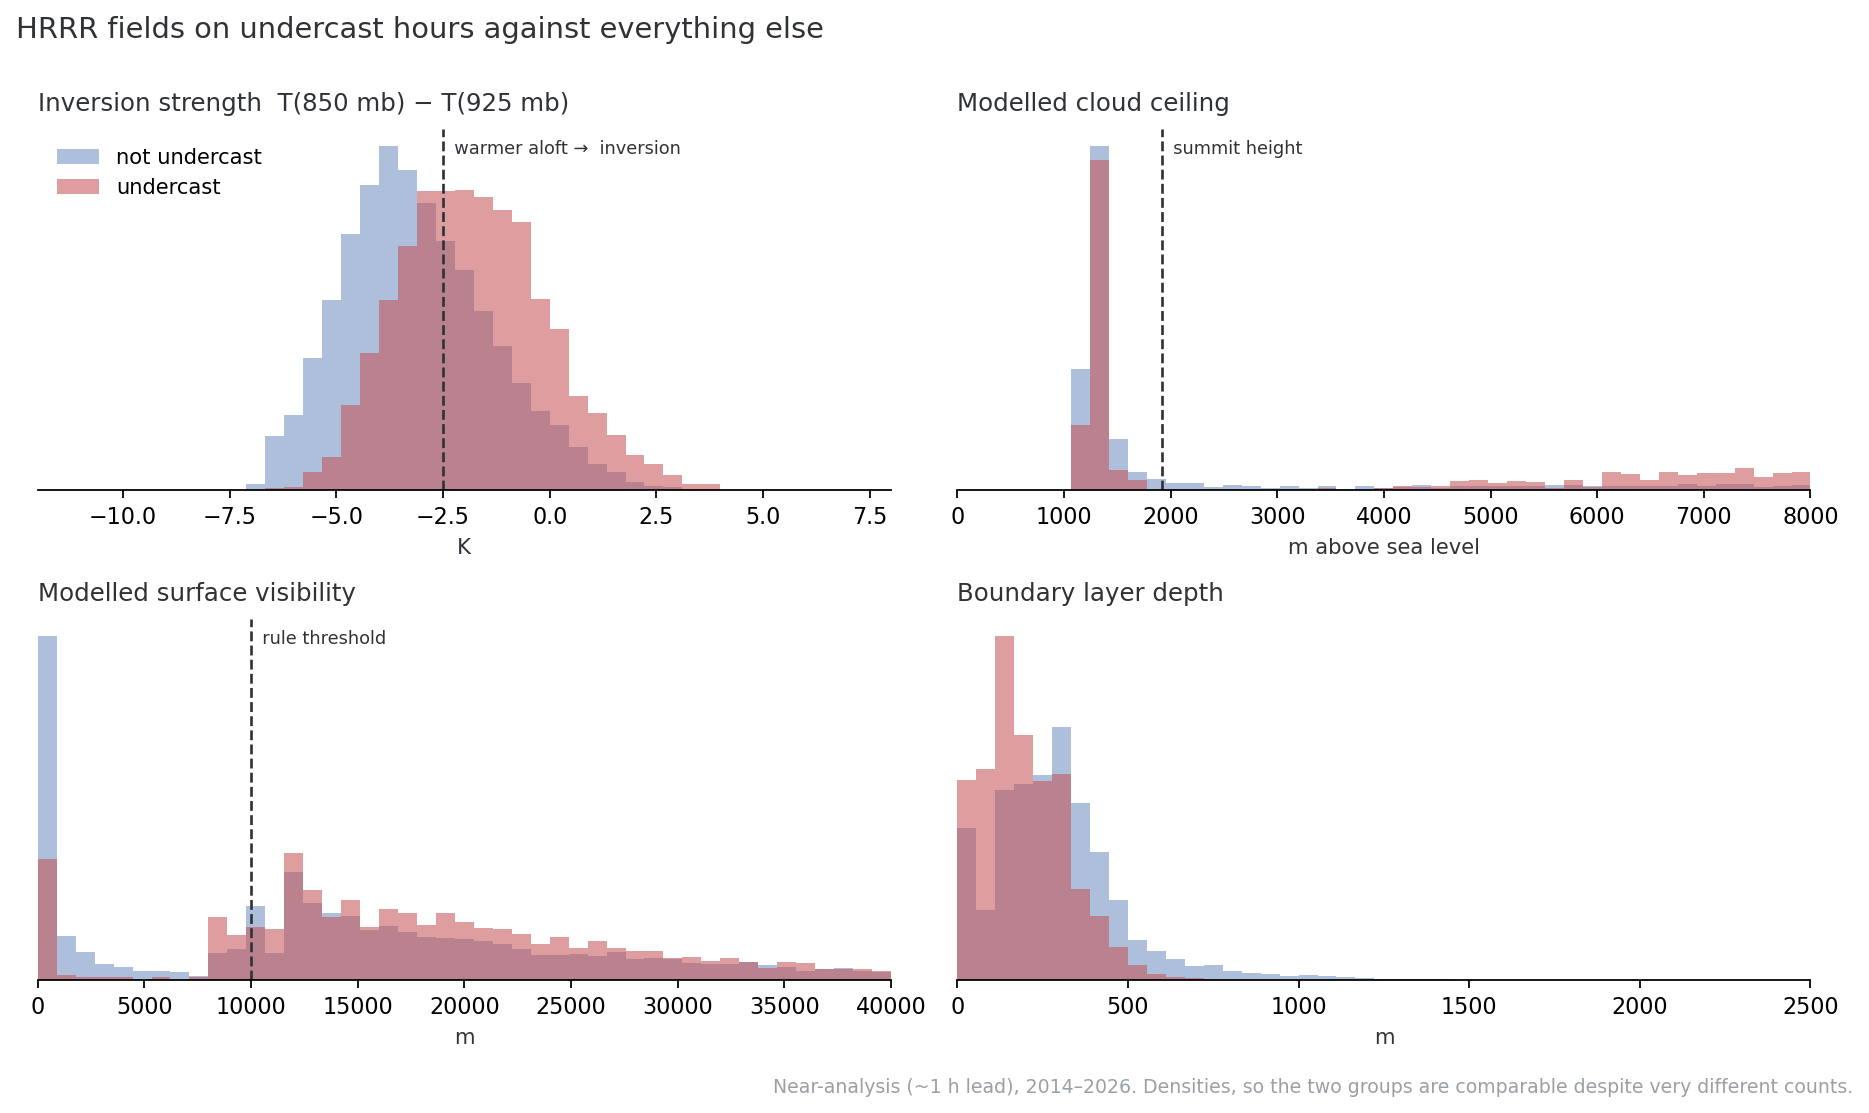
\includegraphics[width=\linewidth]{inversion_evidence.png}
\caption{HRRR fields for undercast hours against all other hours: inversion strength, modelled ceiling,
surface visibility and boundary-layer depth. The spike at zero visibility is the summit in cloud.}\label{fig:inversion}
\end{figure}

%======================================================================
\section{Machine-learning model}\label{sec:ml}
%======================================================================
\subsection{Inputs}
About two dozen fields are taken from every NWP source that publishes them (full list in
\cref{app:features}): cloud cover by layer, cloud base, top and ceiling, temperature and relative
humidity on pressure levels, 2\,m temperature and humidity, boundary-layer height, freezing level,
visibility, wind, precipitation, and derived differences such as summit-minus-925\,mb temperature and
925--850\,mb humidity lapse. Missing values are filled with the constant $-9999$ and get missingness
indicators. Cloud-geometry columns also carry a \code{\_no\_cloud} flag, because a missing value there
means the model reports clear sky, not that data is missing. A separate model is trained for each NWP
source, and a \emph{combined} model uses all sources' columns together (213 features).

\subsection{Algorithms}
Three tree ensembles are trained for each source: Random Forest, Gradient Boosting and XGBoost.
Undercast hours make up about 3\% of the data, and the imbalance is handled with class weights
(balanced weights for the forest and for gradient boosting, \code{scale\_pos\_weight} for XGBoost)
instead of synthetic samples. Given how noisy the labels are, anything more elaborate would mostly fit
labelling error.

\subsection{Validation design}
Neighbouring hours are not independent, so the splits respect time:
\begin{itemize}
\item Cross-validation folds are grouped by week (5 folds), so a multi-day inversion cannot straddle
  the training and test sets.
\item Two holdouts are kept apart by date. Any training row that shares a date with a holdout, or
  falls within one day of it, is dropped (about 17\% of training rows). The \emph{held-out year}
  keeps the true base rate: 16{,}690 hours, 413 of them undercast (2.5\%). The \emph{webcam holdout}
  is the 589 hand-labelled days at all seven leads (4{,}122 forecast rows, 154 undercast).
\item Negatives are subsampled 5:1 in training, which keeps every positive. Training-set precision is
  therefore inflated, so each decision threshold is fitted on the unsampled held-out year: one
  F1-optimal threshold per forecast lead.
\end{itemize}
The combined model trains on 31{,}009 rows (5{,}572 positive) spanning 104 weeks, 2023--2026. The ECMWF
open-data archive starts in 2023, which limits the combined model to those years.
\Cref{fig:leakage} shows why this design matters. A first version split rows at random, so the other
$\sim$23 hours of the same day sat in the training set. That gave precision above 0.9, which was
memorisation, not forecast skill. With date-grouped splits, the same model, data and algorithms reach
about 0.2.

\begin{figure}[ht]\centering
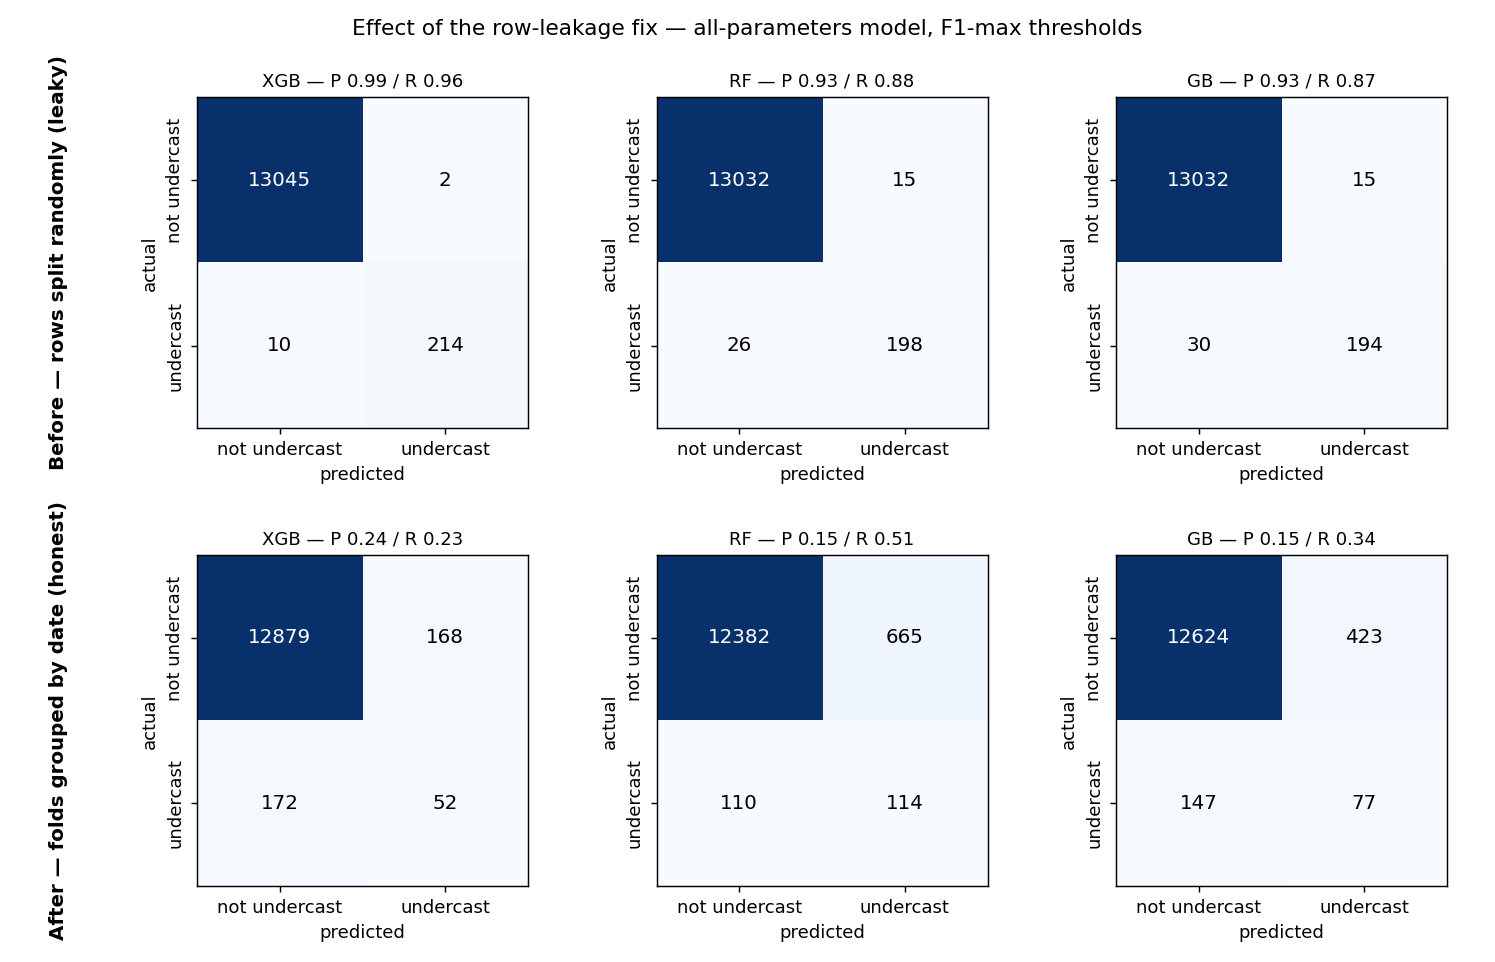
\includegraphics[width=0.8\linewidth]{leakage_before_after.png}
\caption{First-pass all-sources model, out-of-fold, with a row-wise split (top) and a date-grouped
split (bottom). This is the only figure from the first pass and is not comparable with the other
numbers here.}\label{fig:leakage}
\end{figure}

\subsection{Results by source and lead}
Each test row is a forecast issued 1, 24, 48, 72, 96, 120 or 144\,h before its valid time. One model
serves all leads, and each lead gets its own threshold. The combined model beats every individual
source at every lead, and the margin grows with lead time: within 0.05 ROC-AUC of the best single
source at 1\,h, 0.09 ahead at 120\,h (\cref{tab:auclead,fig:lead}). ROC-AUC declines gradually with
lead, while precision drops quickly. \Cref{fig:persource} summarises each source across algorithms,
\cref{fig:rocpr} shows the curves of the combined model and \cref{fig:features} its most important
features. Feature importances are hard to interpret, because many columns are strongly correlated
(\cref{sec:overfit}). Even so, ECMWF moisture structure (925--850\,mb RH difference) ranks first under
every algorithm.

\begin{table}[ht]\centering\small
\caption{ROC-AUC on the held-out year by forecast lead, Gradient Boosting. A dash means the source
does not reach that lead.}\label{tab:auclead}
\begin{tabular}{l r r r r r r r}
\toprule
Source & 1\,h & 24\,h & 48\,h & 72\,h & 96\,h & 120\,h & 144\,h\\
\midrule
\textbf{Combined} & \textbf{0.941} & \textbf{0.922} & \textbf{0.880} & \textbf{0.857} & \textbf{0.824} & \textbf{0.775} & \textbf{0.764}\\
RAP   & 0.890 & 0.859 & 0.804 & --- & --- & --- & ---\\
HRRR  & 0.889 & 0.870 & 0.837 & --- & --- & --- & ---\\
ECMWF & 0.879 & 0.872 & 0.842 & 0.847 & 0.804 & 0.739 & 0.754\\
NAM   & 0.861 & 0.830 & 0.818 & --- & --- & --- & ---\\
NBM   & 0.844 & 0.769 & 0.762 & 0.734 & 0.690 & 0.675 & 0.651\\
GFS   & 0.842 & 0.818 & 0.790 & 0.747 & 0.745 & 0.682 & ---\\
\bottomrule
\end{tabular}
\end{table}

\begin{figure}[ht]\centering
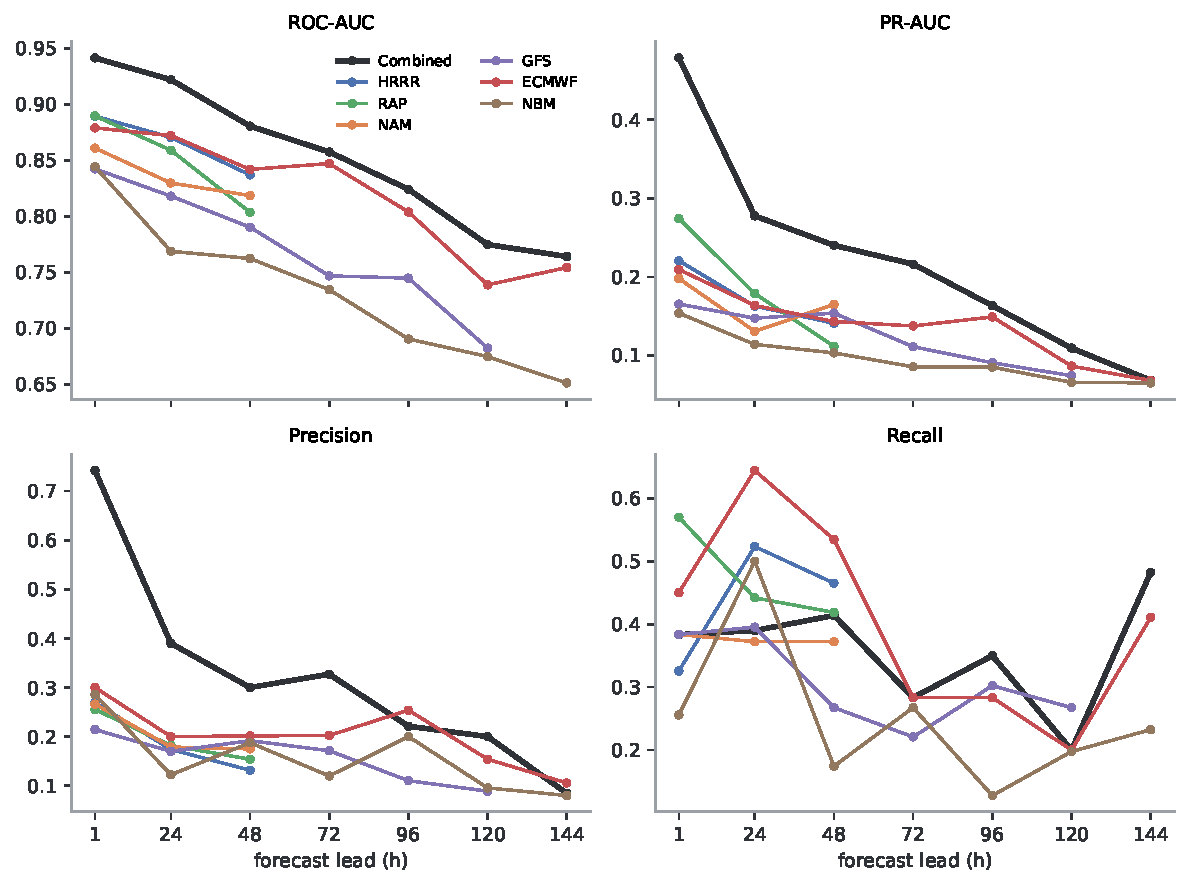
\includegraphics[width=0.85\linewidth]{skill_vs_lead.pdf}
\caption{Skill against forecast lead on the held-out year, Gradient Boosting, each lead at its own
threshold. The combined model is the heavy line.}\label{fig:lead}
\end{figure}

\begin{figure}[ht]\centering
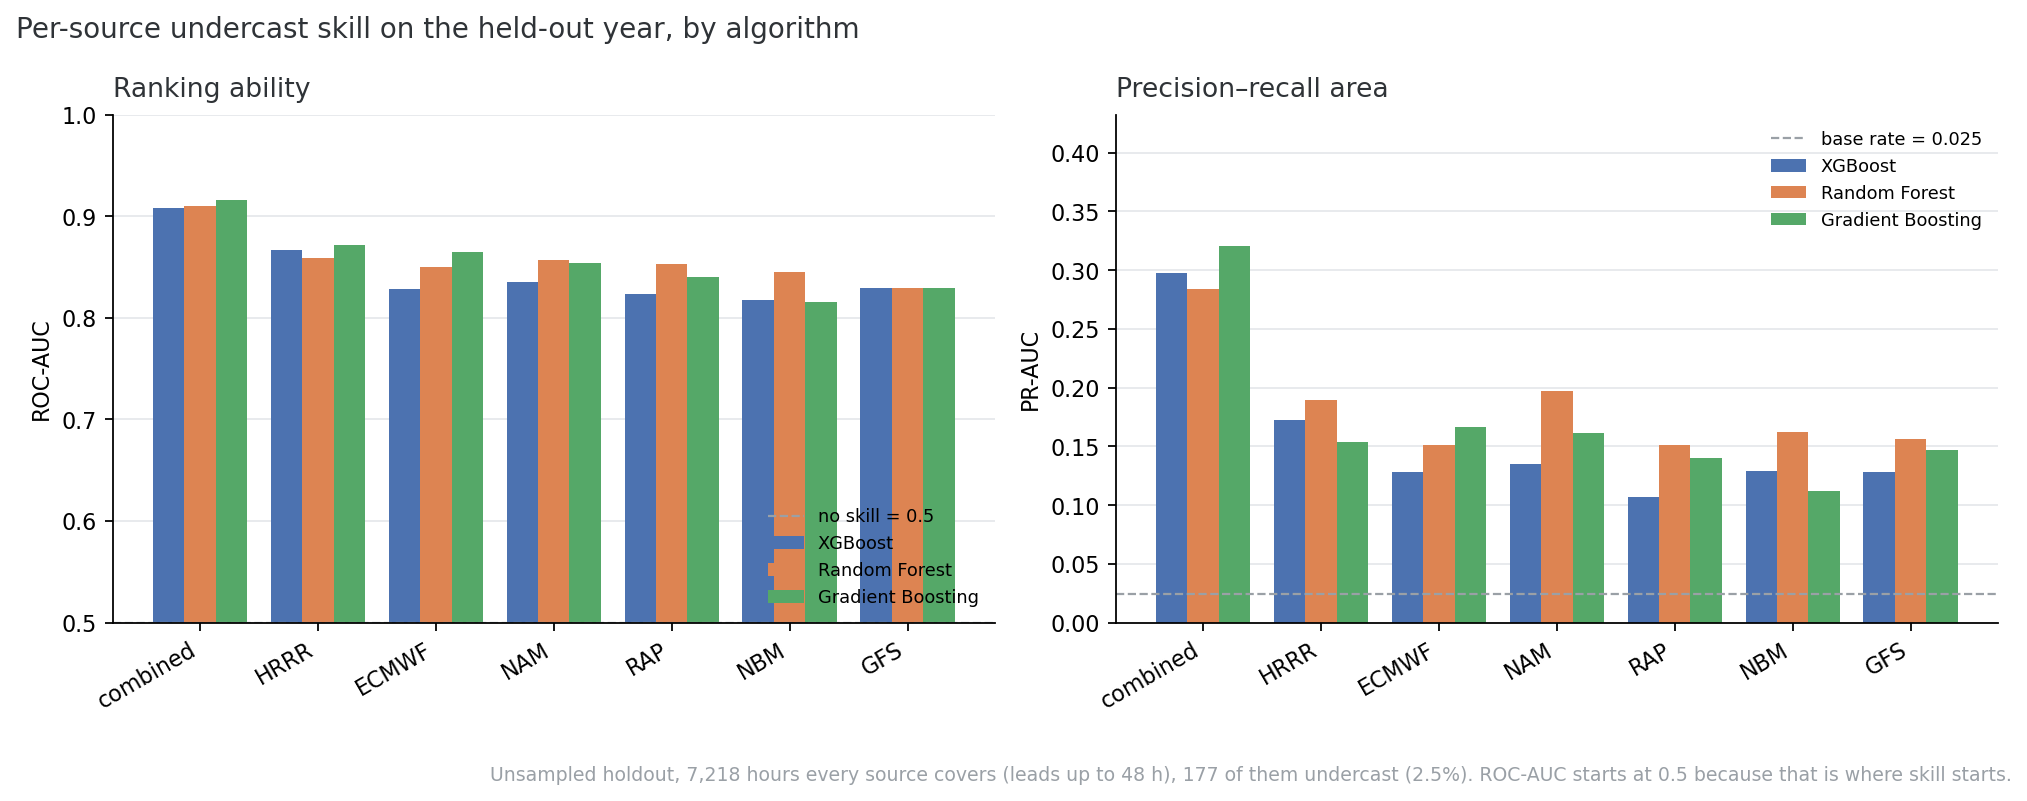
\includegraphics[width=0.85\linewidth]{per_source_performance.png}
\caption{ROC-AUC and PR-AUC for each source on the held-out year. ``Mean of 3'' averages the three
algorithms' probabilities.}\label{fig:persource}
\end{figure}

\begin{figure}[ht]\centering
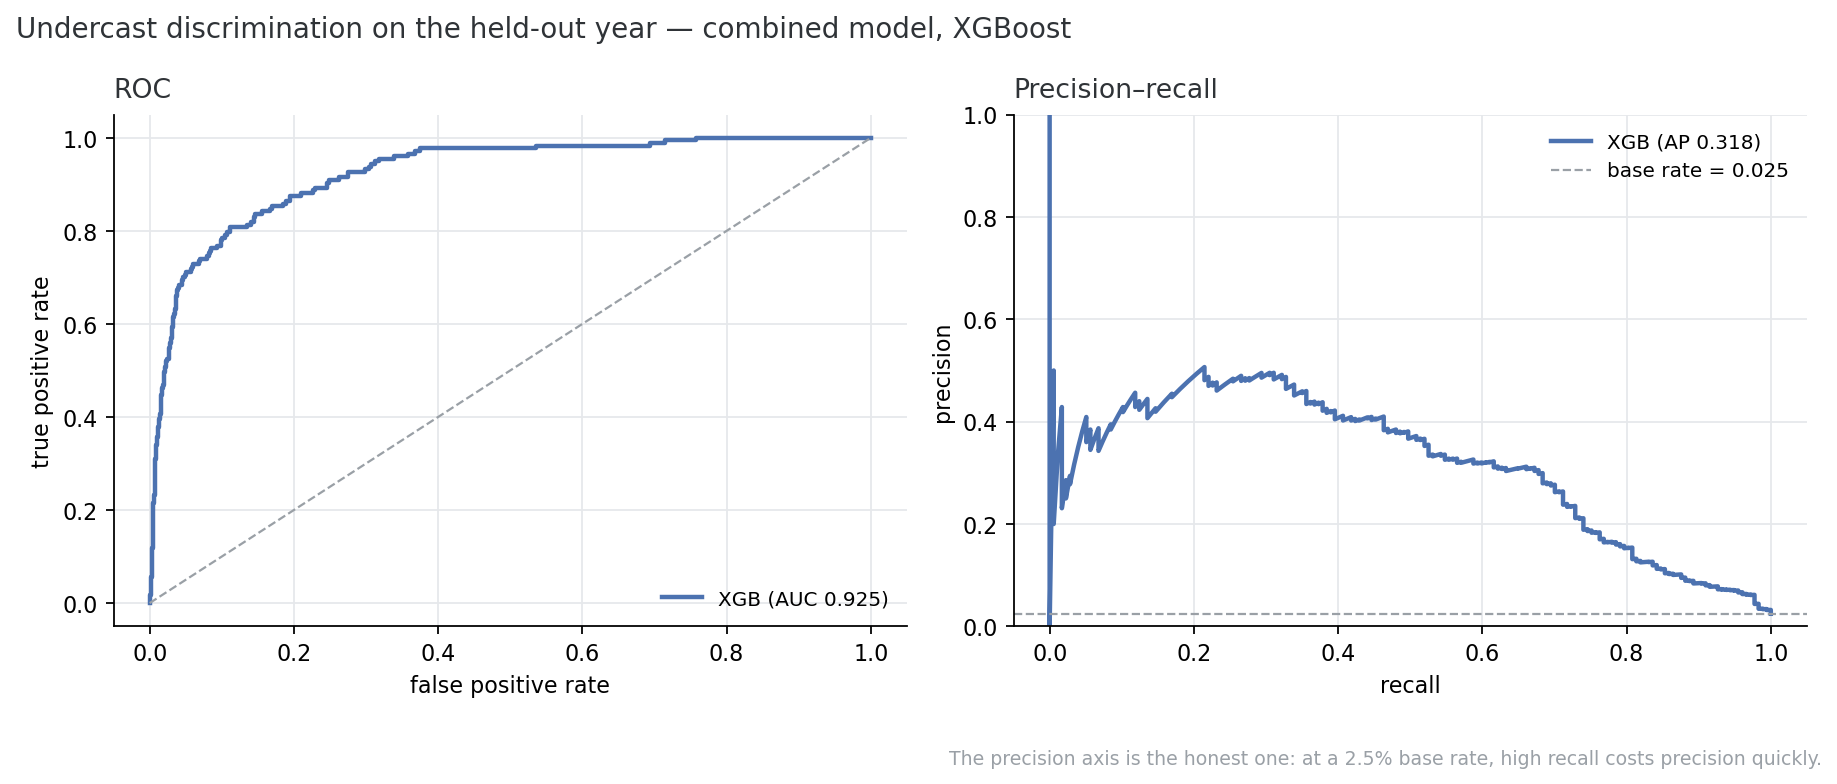
\includegraphics[width=0.32\linewidth]{roc_pr_curves_all_xgboost.png}\hfill
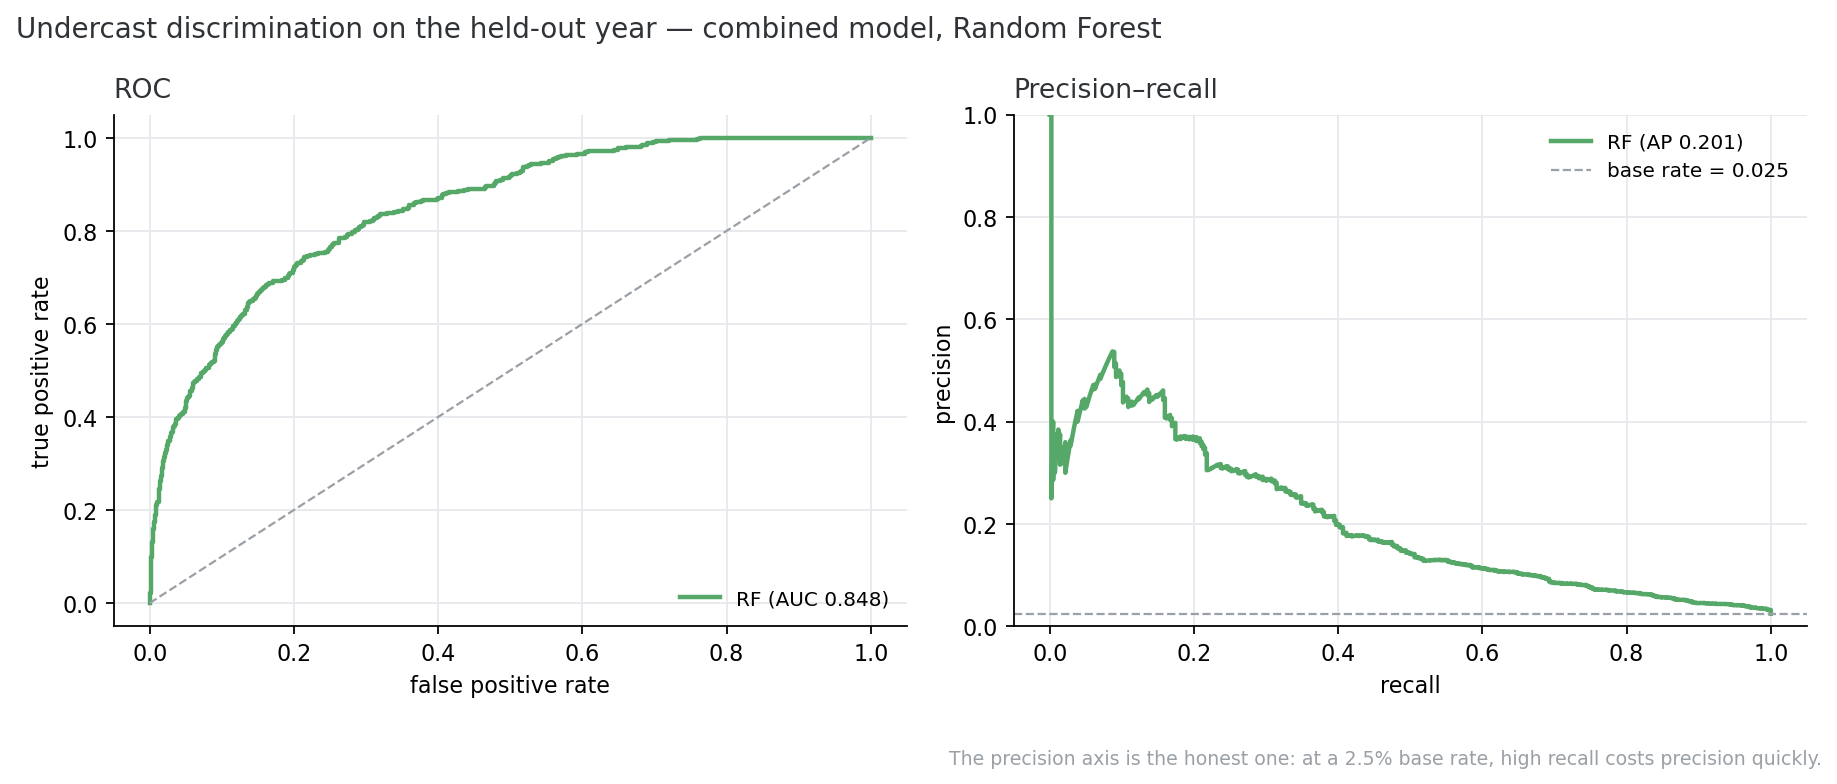
\includegraphics[width=0.32\linewidth]{roc_pr_curves_all_random_forest.png}\hfill
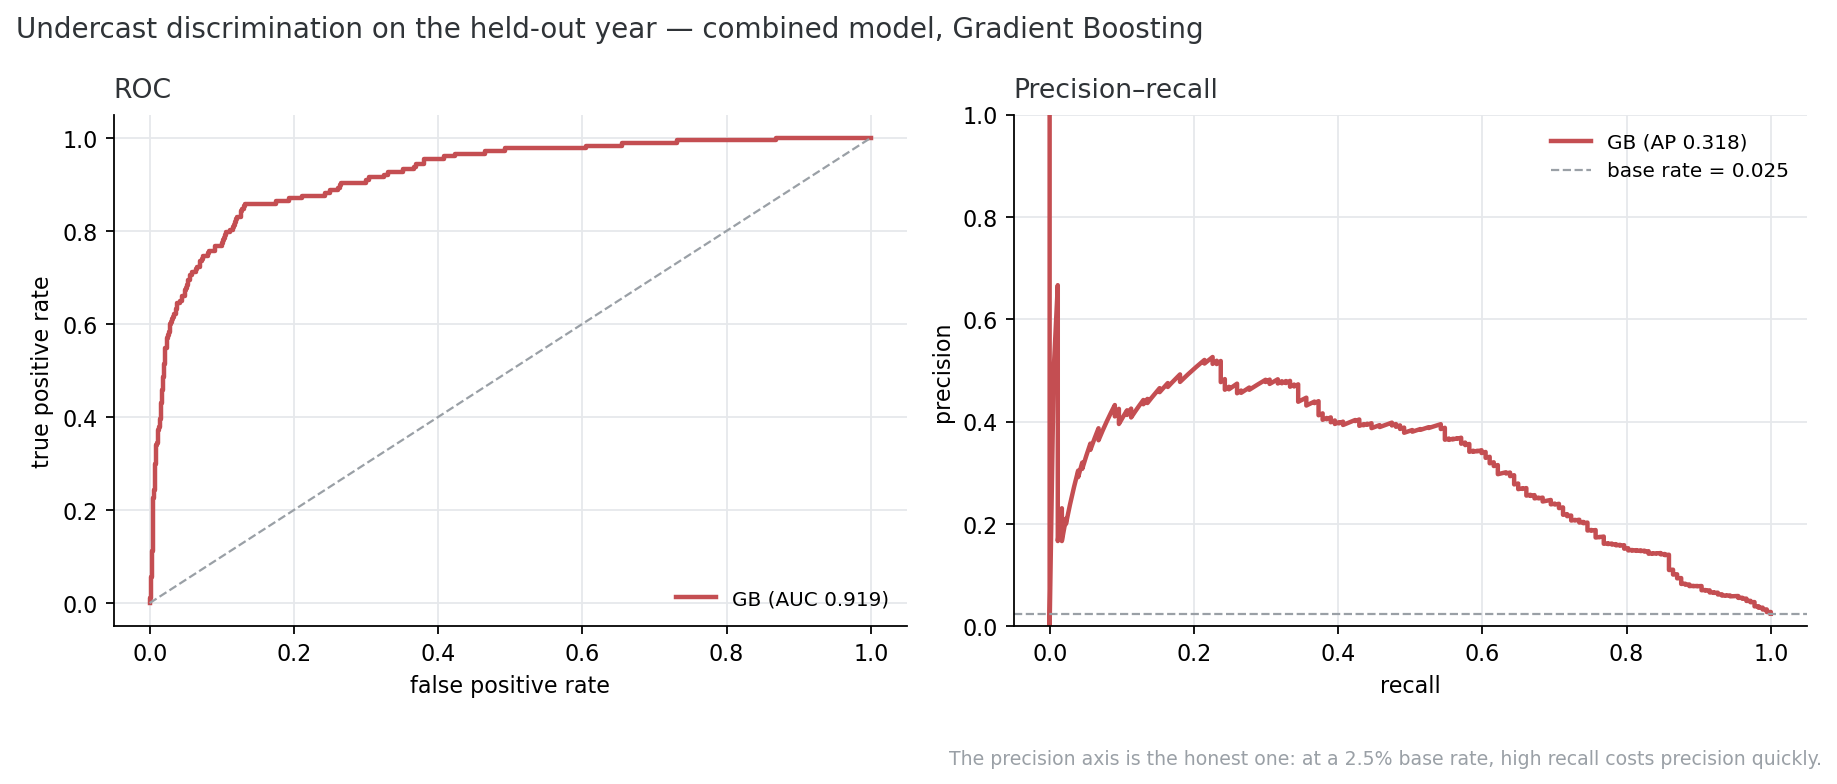
\includegraphics[width=0.32\linewidth]{roc_pr_curves_all_gradient_boosting.png}
\caption{ROC and precision--recall curves of the combined model on the held-out year: XGBoost, Random
Forest, Gradient Boosting (left to right). The three finish within 0.03 ROC-AUC of each other.}\label{fig:rocpr}
\end{figure}

\begin{figure}[ht]\centering
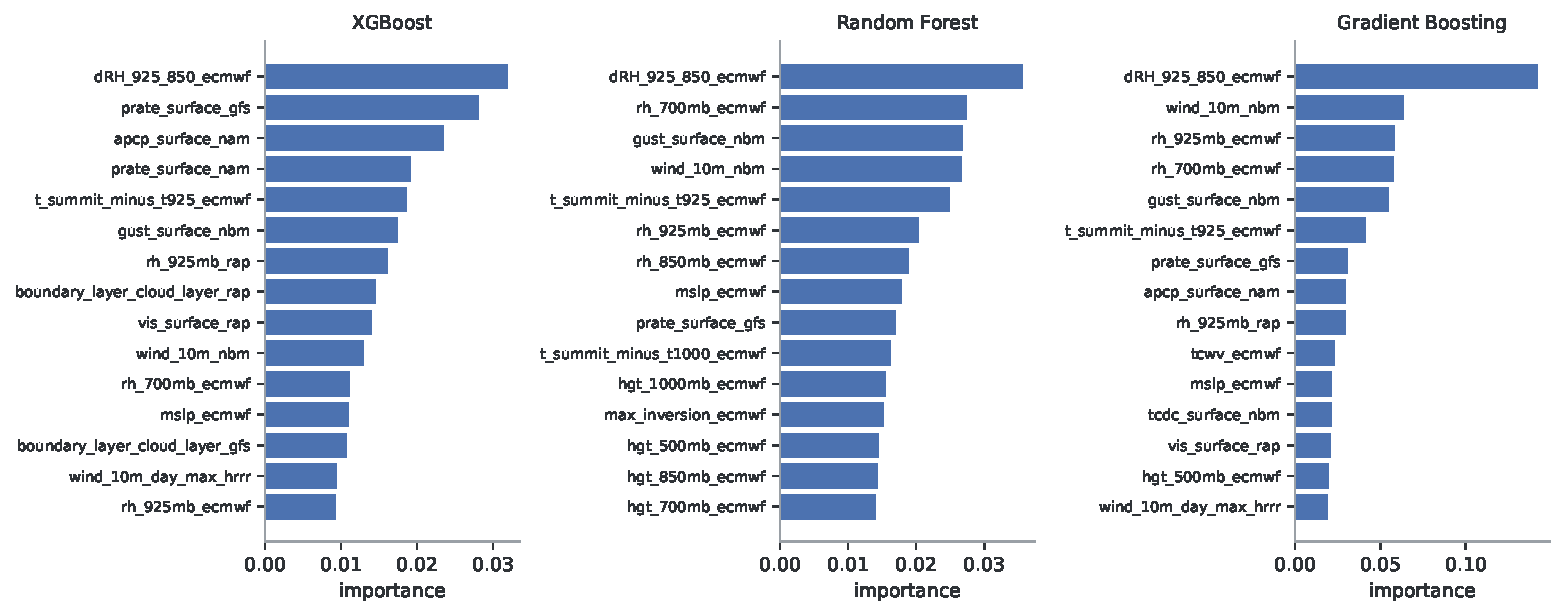
\includegraphics[width=\linewidth]{features_combined.pdf}
\caption{Top 15 feature importances of the combined model for each algorithm. Per-source importances
are in \cref{app:sources}.}\label{fig:features}
\end{figure}

\subsection{Choice of algorithm}
An ensemble only helps when its members make different mistakes. On one NWP source, the three
algorithms' predictions have rank correlations of 0.86--0.95. The six NWP sources under one algorithm
correlate at only 0.34--0.58 (\cref{fig:diversity}). Accordingly, voting across algorithms gains
nothing (\cref{tab:vote}), and neither do four alternative algorithms (\cref{tab:alt}). The
disagreement worth exploiting is between NWP sources: the combined model reaches ROC-AUC 0.908
[0.860, 0.951], $+0.013$ [$+0.003$, $+0.026$] above the average of the six single-source models
(95\% intervals from a bootstrap over days; \cref{fig:diversity}, right). The production model is therefore a
single combined-source Gradient Boosting model with per-lead thresholds.

\begin{figure}[ht]\centering
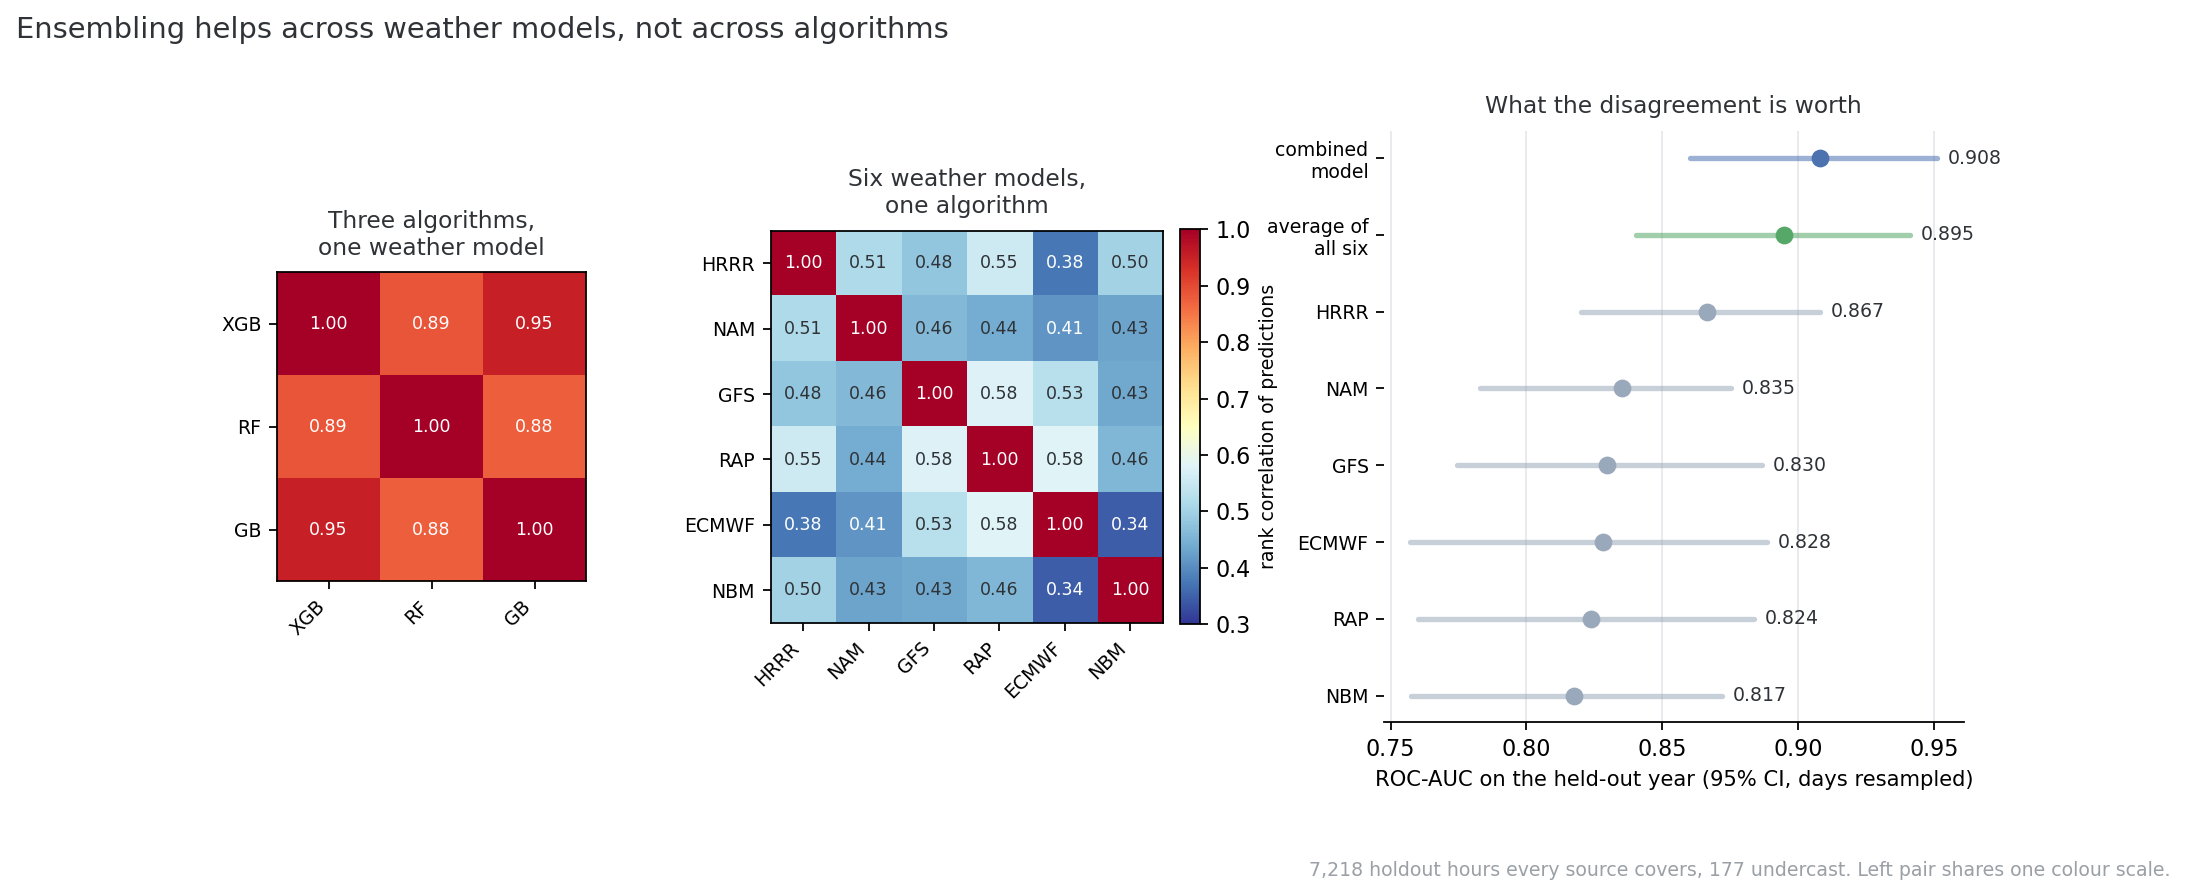
\includegraphics[width=\linewidth]{ensemble_diversity.png}
\caption{Rank correlation between algorithms (left) and between NWP sources (middle), on a shared
colour scale; ROC-AUC with bootstrap 95\% intervals (right).}\label{fig:diversity}
\end{figure}

\begin{table}[ht]\centering\small
\caption{Combined model, each algorithm at its own F1-optimal threshold.}\label{tab:vote}
\begin{tabular}{l rrr rrr}
\toprule
& \multicolumn{3}{c}{Held-out year} & \multicolumn{3}{c}{Webcam days}\\
\cmidrule(lr){2-4}\cmidrule(lr){5-7}
Predictor & P & R & F1 & P & R & F1\\
\midrule
XGBoost & 0.26 & 0.29 & 0.27 & 0.35 & 0.18 & 0.24\\
Random Forest & 0.28 & 0.31 & 0.30 & 0.25 & 0.06 & 0.10\\
Gradient Boosting & 0.28 & 0.32 & 0.30 & 0.41 & 0.25 & 0.31\\
Any of the three & 0.22 & 0.39 & 0.28 & 0.36 & 0.28 & 0.32\\
2 of 3 (vote) & 0.31 & 0.30 & 0.30 & 0.38 & 0.17 & 0.23\\
Unanimous & 0.37 & 0.24 & 0.29 & 0.28 & 0.05 & 0.09\\
Mean probability & 0.28 & 0.31 & 0.29 & 0.31 & 0.14 & 0.19\\
\bottomrule
\end{tabular}
\end{table}

\begin{table}[ht]\centering\small
\caption{ROC-AUC on the held-out year for other algorithms. Histogram gradient boosting gets the raw
columns, since it splits on missing values natively. Logistic regression gets median imputation and
standardisation.}\label{tab:alt}
\begin{tabular}{l r r}
\toprule
Algorithm & Combined & HRRR\\
\midrule
Gradient Boosting & 0.862 & 0.866\\
Random Forest, deeper trees & 0.849 & 0.855\\
Random Forest & 0.848 & 0.862\\
XGBoost & 0.843 & 0.863\\
Logistic regression & 0.819 & 0.861\\
Histogram gradient boosting & 0.819 & 0.854\\
Extra Trees & 0.799 & 0.850\\
\bottomrule
\end{tabular}
\end{table}

\subsection{Overfitting checks}\label{sec:overfit}
The combined model has 213 feature columns, and its training rows are far from independent. Each
undercast hour appears once per lead, and consecutive hours belong to the same event
(\cref{tab:units}). There are more feature columns than distinct undercast days.

\begin{table}[ht]\centering\small
\caption{Effective size of the combined model's training set.}\label{tab:units}
\begin{tabular}{l r r}
\toprule
Counting unit & $n$ & Per feature\\
\midrule
Positive rows & 5{,}572 & 26.2\\
Distinct positive valid hours (leads de-duplicated) & 797 & 3.7\\
Distinct undercast episodes (gaps $\le2$\,h bridged) & 182 & 0.85\\
Distinct undercast days & 175 & 0.82\\
\bottomrule
\end{tabular}
\end{table}

The features are just as redundant. The 213 columns represent 78 physical quantities plus four
calendar encodings (82 in total). Of the physical quantities, 41 come from more than one source and
37 from only one. The median $|\text{Spearman } r|$ between the same quantity from different sources
is 0.872, against 0.181 for random pairs of different quantities (\cref{fig:redundancy}). A principal
component analysis of the 11{,}620 training rows where every source reports, over the 98 columns
populated more than half the time, needs 21 components for 90\% of the variance and 29 for 95\%. The
participation ratio is 8.7.

Directly reducing model capacity does not help (\cref{fig:trimdepth}). Keeping only the top $k$
features matches the full model at $k\ge70$ and loses up to 0.05 ROC-AUC below that. A maximum tree
depth of 3 is as good as any other within the $\pm0.005$ reseed noise.

\begin{figure}[ht]\centering
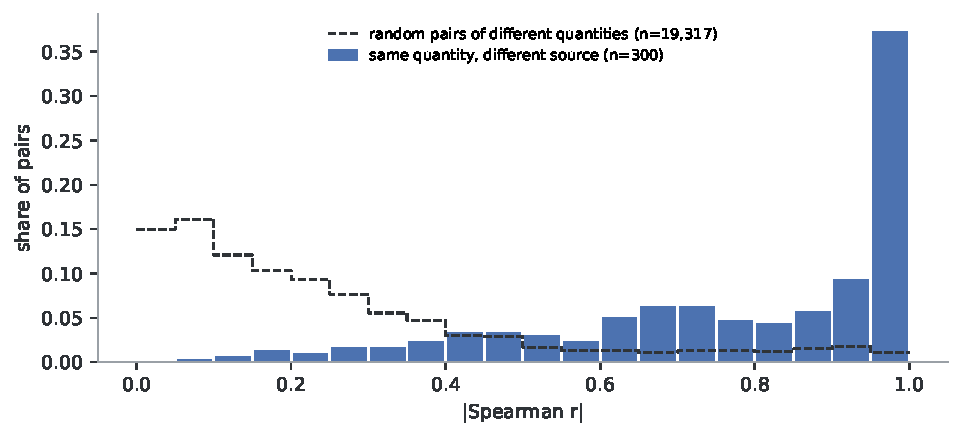
\includegraphics[width=0.7\linewidth]{redundancy_hist.pdf}
\caption{$|\text{Spearman } r|$ for all 300 same-quantity, different-source pairs (bars) against
19{,}317 random pairs of different quantities (dashed), each as a share of its own total.}\label{fig:redundancy}
\end{figure}

\begin{figure}[ht]\centering
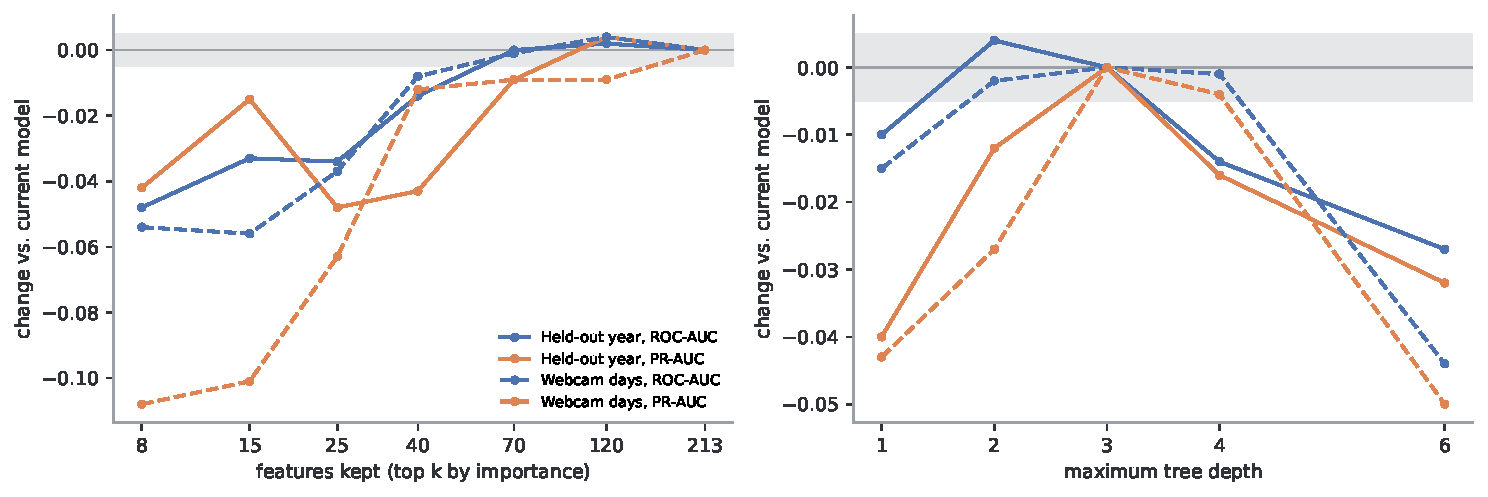
\includegraphics[width=\linewidth]{trim_depth.pdf}
\caption{Change in ROC-AUC and PR-AUC against the production configuration when keeping only the top
$k$ features (left) or changing the maximum tree depth (right), on both holdouts. The grey band is
the $\pm0.005$ spread over five seeds.}\label{fig:trimdepth}
\end{figure}

\subsection{Production model}
The production forecast is a Gradient Boosting model with maximum depth 3, trained on all 213 combined
features, with a separate threshold for each lead. \Cref{tab:final} gives the held-out-year results
that the website's Model performance panel shows, and \cref{fig:final} gives the confusion matrices.
At 1\,h, three of every four undercast calls are right. At 24\,h it is about two in five, and at
144\,h about one in twelve.

\begin{table}[ht]\centering\small
\caption{Production model on the held-out year (true base rate), by forecast lead.}\label{tab:final}
\begin{tabular}{r r r r r r r r r r}
\toprule
Lead (h) & Threshold & Hours & Undercast & TP & FP & FN & Precision & Recall & ROC-AUC\\
\midrule
1   & 0.880 & 2{,}397 & 60 & 23 & 8   & 37 & 0.74 & 0.38 & 0.941\\
24  & 0.835 & 2{,}414 & 59 & 23 & 36  & 36 & 0.39 & 0.39 & 0.922\\
48  & 0.805 & 2{,}407 & 58 & 24 & 56  & 34 & 0.30 & 0.41 & 0.880\\
72  & 0.815 & 2{,}408 & 60 & 17 & 35  & 43 & 0.33 & 0.28 & 0.857\\
96  & 0.735 & 2{,}384 & 60 & 21 & 74  & 39 & 0.22 & 0.35 & 0.824\\
120 & 0.780 & 2{,}377 & 60 & 12 & 48  & 48 & 0.20 & 0.20 & 0.775\\
144 & 0.620 & 2{,}303 & 56 & 27 & 293 & 29 & 0.08 & 0.48 & 0.764\\
\bottomrule
\end{tabular}
\end{table}

\begin{figure}[ht]\centering
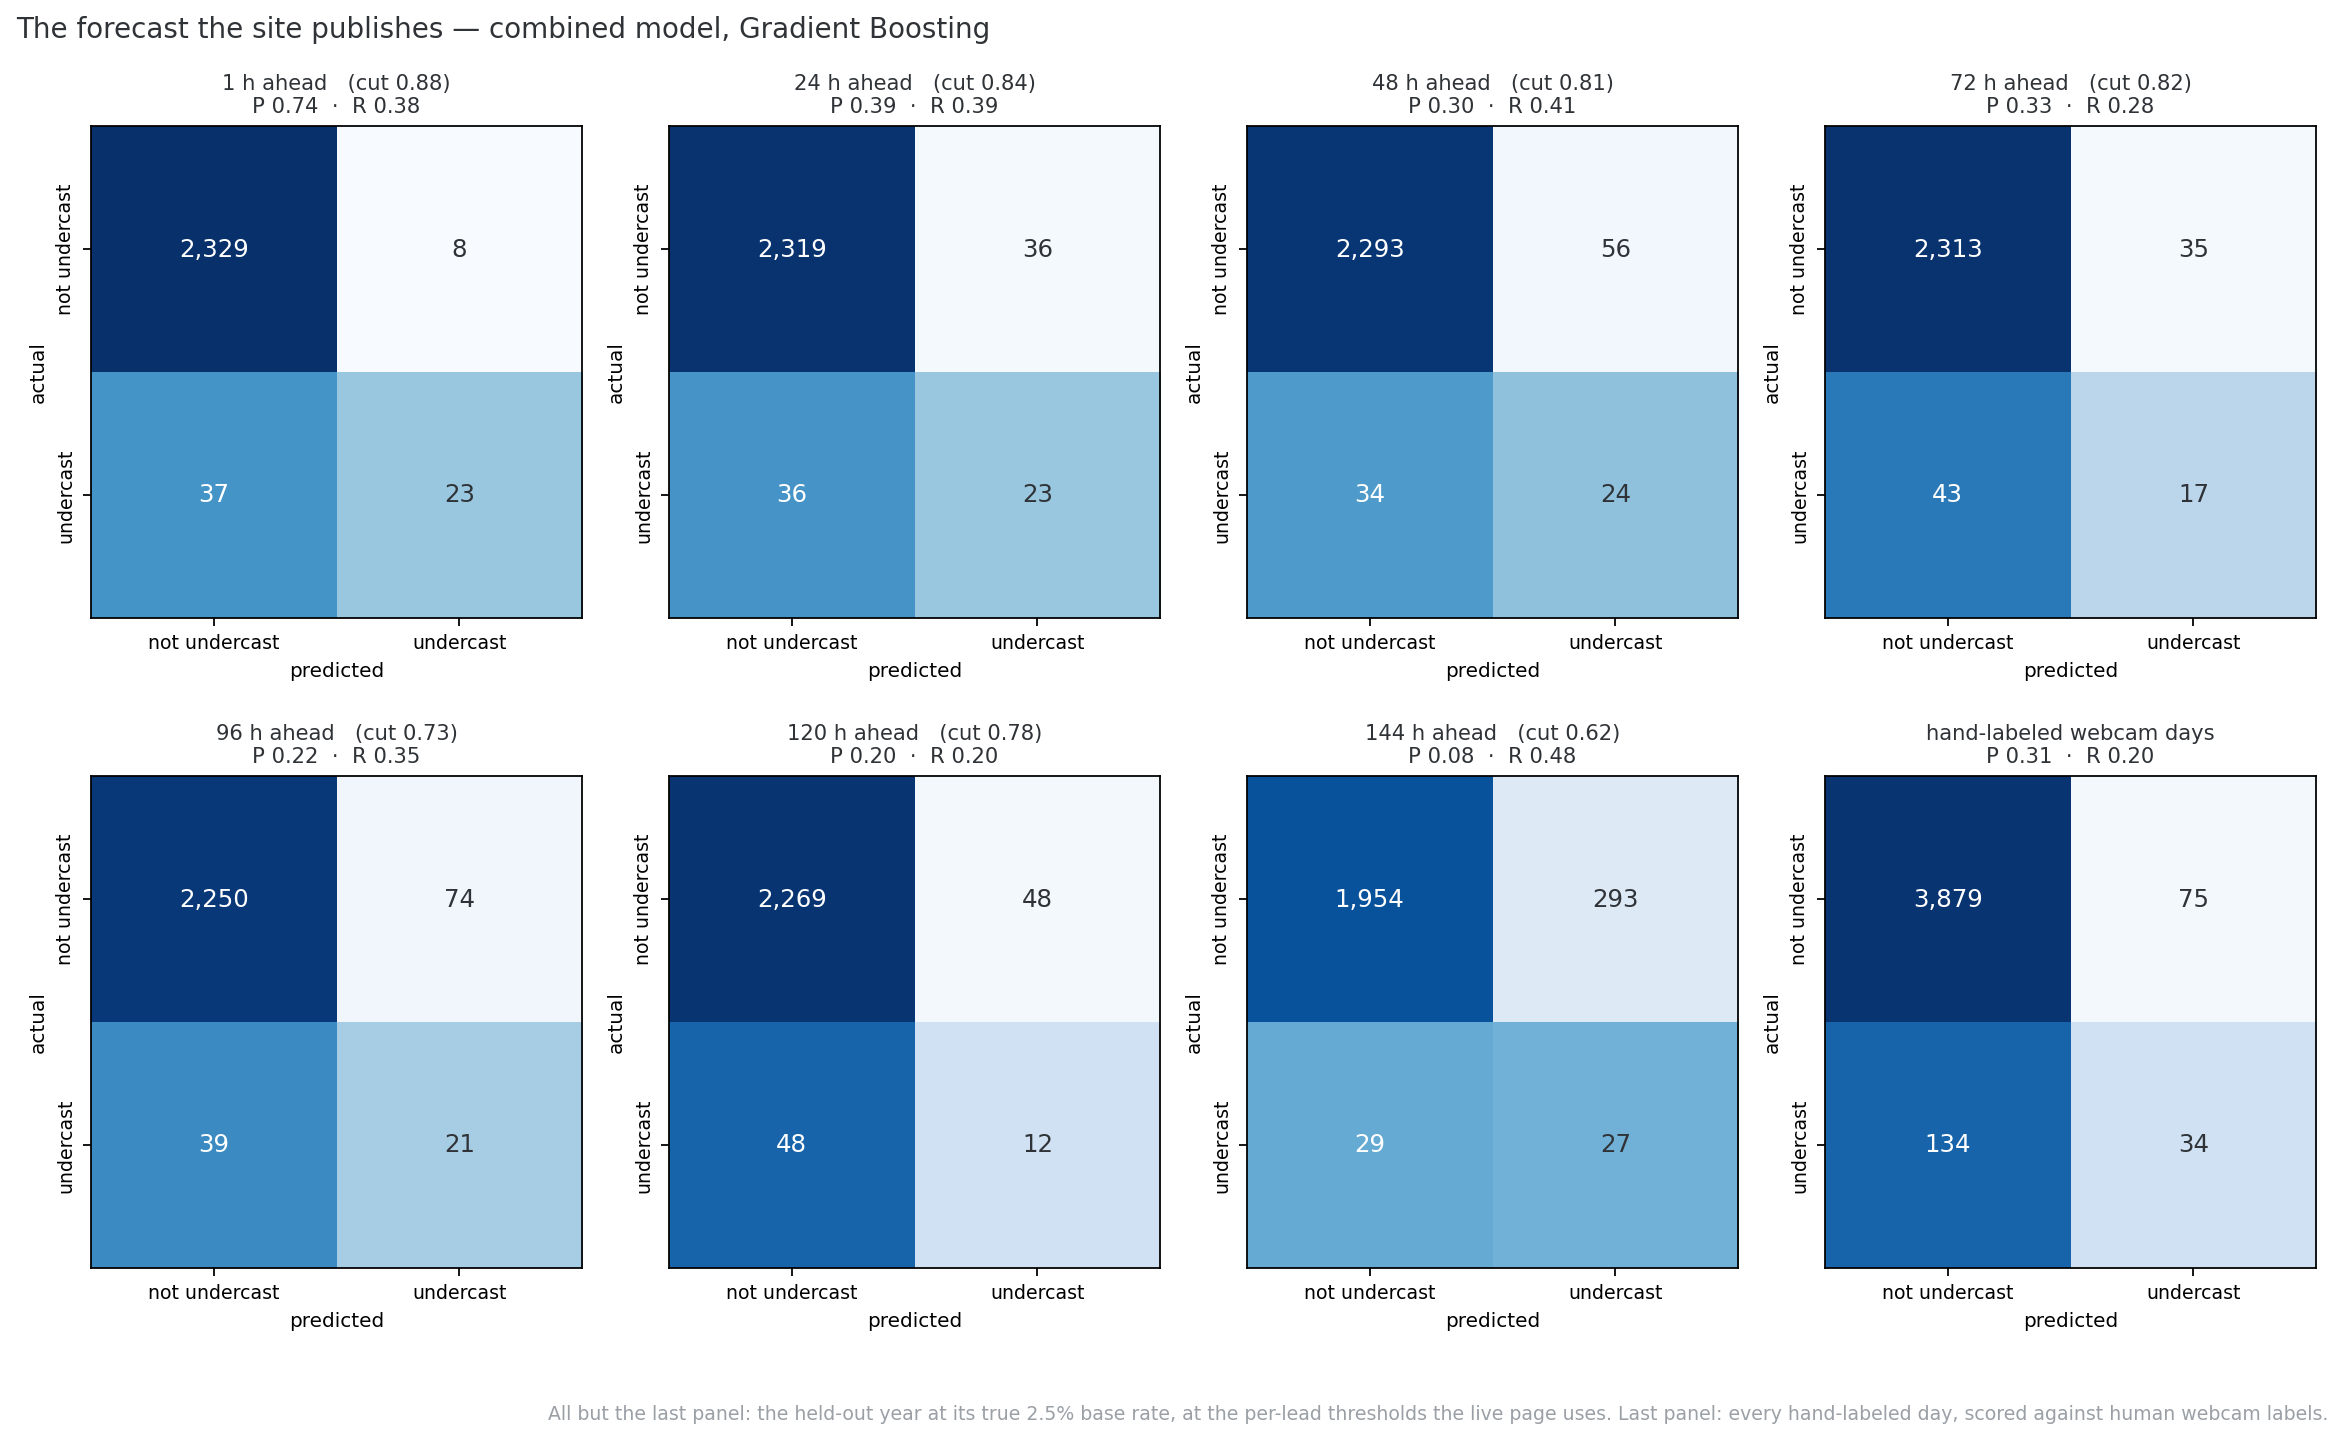
\includegraphics[width=\linewidth]{headline_model_confusion.png}
\caption{Production model confusion matrices at each lead on the held-out year, and on the webcam
days.}\label{fig:final}
\end{figure}

%======================================================================
\section{Limitations and next steps}\label{sec:limits}
%======================================================================
\begin{itemize}
\item \textbf{Labels set the ceiling.} The remark cuts are about 70\% precise, so roughly three in
  ten training positives are not real undercasts. No classifier can be much cleaner than its target.
  The webcam set behind that estimate has only 22 positive days.
\item \textbf{Reporting drift.} The pass rate quadruples over 1997--2026, most likely because of
  changing observer practice. Matched sampling removes the calendar signal, but the label definition
  is not stationary.
\item \textbf{Vertical resolution.} The pressure levels used are 1000, 925, 850, 700 and 500\,mb.
  The 1{,}564\,m gap between 850 and 700\,mb straddles the 1{,}917\,m summit, so the top of the
  inversion can only be interpolated. Fetching 800 and 750\,mb fields would bracket it.
\item \textbf{Observed profiles.} The MWOBS mesonet includes an Auto Road Vertical Profile: six
  stations from 1{,}600 to 5{,}300\,ft plus the summit tower, with 5-minute temperature, humidity,
  wind and solar radiation~\cite{fowler}. It would measure the inversion directly. Synoptic Data holds
  it only from 18~February~2026, so earlier history must be requested from MWOBS.
\item \textbf{Not yet explored.} The effect of the 5:1 negative subsampling ratio, and which physical
  factors drive the per-source differences.
\end{itemize}

\FloatBarrier
\section*{Data, code and AI use}
All scripts are in the repository \url{https://github.com/lucasehinger/lucasehinger.github.io}
(\code{scripts/}). Model metadata and metrics are in \code{files/weather/models/obs/}. Figures in this
document come from the website or from \code{scripts/build\_weather\_report\_figures.py}. For data
access, contact \href{mailto:ehingerl@mit.edu}{ehingerl@mit.edu}. NWP data is from NOAA and ECMWF,
accessed with the Herbie Python package. Webcam imagery and METAR remarks are from the Mount Washington
Observatory. Most of the code was written with AI assistance. The author made the modelling decisions
and reviewed every analysis step, and wrote most of the website text.

\begin{thebibliography}{9}\small
\bibitem{mwobs} Mount Washington Observatory, ``Undercast,'' \url{https://mountwashington.org/undercast/}.
\bibitem{gmc} Green Mountain Club, ``Temperature inversion \& undercast,'' \url{https://www.greenmountainclub.org/temperature-inversion-undercast-obsession/}.
\bibitem{sd} \emph{Atmospheric Research}, \url{https://www.sciencedirect.com/science/article/abs/pii/S016980951930941X}.
\bibitem{blm} \emph{Boundary-Layer Meteorology}, \url{https://doi.org/10.1007/s10546-009-9407-1}.
\bibitem{esw} EatSleepWild, ``What is a cloud inversion?'' \url{https://eatsleepwild.com/what-is-a-cloud-inversion/}.
\bibitem{fowler} Fowler \emph{et al.}, \emph{J.\ Atmos.\ Oceanic Technol.}\ \textbf{40}, 439 (2023): the Mount Washington Observatory regional mesonet.
\end{thebibliography}

\clearpage
\appendix
\sloppy
%======================================================================
\section{Website controls and links}\label{app:links}
%======================================================================
The summit selector on the forecast page loads quick links for the selected summit from
\code{files/weather/links/<summit>.json}. For Mount Washington these are the NWS point forecast,
the NWS hourly graph, the NWS Gray, ME area forecast discussion, Windy, the MWOBS Higher Summits
Forecast and the Mount Washington Avalanche Center. The other summits get the same six links, with the NWS and Windy
links pointed at that summit. The details page also has interactive pickers: an algorithm and source picker for
feature importances (\cref{app:sources}), a metric picker for skill against lead (\cref{fig:lead}),
and a lead and source picker for confusion matrices (\cref{tab:persource}). The historical-conditions
page has a date, model and unit picker for the day-by-day NWP viewer.

%======================================================================
\section{Per-source and per-algorithm results}\label{app:sources}
%======================================================================
\begin{table}[ht]\centering\small
\caption{Single-source and combined models, Gradient Boosting. Out-of-fold (OOF) AUCs are from
week-grouped 5-fold cross-validation on the 5:1 subsampled training set. Held-out precision and
recall use the single all-lead threshold.}\label{tab:persource}
\begin{tabular}{l r r r r r r r r}
\toprule
& \multicolumn{3}{c}{Training} & \multicolumn{2}{c}{OOF} & \multicolumn{3}{c}{Held-out year}\\
\cmidrule(lr){2-4}\cmidrule(lr){5-6}\cmidrule(lr){7-9}
Source & Years & Rows & Features & ROC & PR & Thr. & P & R\\
\midrule
Combined & 2023--26 & 31{,}009 & 213 & 0.781 & 0.485 & 0.78 & 0.28 & 0.32\\
HRRR  & 2014--26 & 34{,}829 & 46 & 0.855 & 0.549 & 0.67 & 0.16 & 0.48\\
RAP   & 2021--26 & 16{,}707 & 39 & 0.800 & 0.447 & 0.70 & 0.19 & 0.43\\
NAM   & 2020--26 & 15{,}607 & 38 & 0.820 & 0.475 & 0.73 & 0.19 & 0.39\\
GFS   & 2021--26 & 33{,}990 & 39 & 0.736 & 0.372 & 0.65 & 0.13 & 0.35\\
ECMWF & 2023--26 & 31{,}013 & 40 & 0.722 & 0.374 & 0.66 & 0.16 & 0.49\\
NBM   & 2020--26 & 50{,}097 & 31 & 0.687 & 0.320 & 0.70 & 0.13 & 0.20\\
\bottomrule
\end{tabular}
\end{table}

\begin{table}[ht]\centering\small
\caption{Held-out-year precision\,/\,recall by lead for each source, Gradient Boosting, each lead at
its own threshold.}\label{tab:prlead}
\begin{tabular}{l c c c c c c c}
\toprule
Source & 1\,h & 24\,h & 48\,h & 72\,h & 96\,h & 120\,h & 144\,h\\
\midrule
Combined & .74/.38 & .39/.39 & .30/.41 & .33/.28 & .22/.35 & .20/.20 & .08/.48\\
HRRR  & .27/.33 & .17/.52 & .13/.47 & --- & --- & --- & ---\\
RAP   & .26/.57 & .18/.44 & .15/.42 & --- & --- & --- & ---\\
NAM   & .27/.38 & .18/.37 & .17/.37 & --- & --- & --- & ---\\
GFS   & .21/.38 & .17/.40 & .19/.27 & .17/.22 & .11/.30 & .09/.27 & ---\\
ECMWF & .30/.45 & .20/.64 & .20/.53 & .20/.28 & .25/.28 & .15/.20 & .11/.41\\
NBM   & .29/.26 & .12/.50 & .19/.17 & .12/.27 & .20/.13 & .10/.20 & .08/.23\\
\bottomrule
\end{tabular}
\end{table}

\begin{table}[ht]\centering\small
\caption{Combined model by algorithm and lead on the held-out year: ROC-AUC, precision\,/\,recall.}\label{tab:algolead}
\begin{tabular}{l c c c c c c c}
\toprule
Algorithm & 1\,h & 24\,h & 48\,h & 72\,h & 96\,h & 120\,h & 144\,h\\
\midrule
XGBoost & 0.940 & 0.907 & 0.871 & 0.836 & 0.789 & 0.753 & 0.724\\
        & .60/.50 & .32/.49 & .24/.52 & .21/.35 & .20/.18 & .10/.32 & .09/.21\\
Random Forest & 0.938 & 0.911 & 0.876 & 0.839 & 0.797 & 0.774 & 0.726\\
        & .54/.57 & .33/.51 & .28/.47 & .30/.25 & .22/.35 & .24/.17 & .07/.39\\
Gradient Boosting & 0.941 & 0.922 & 0.880 & 0.857 & 0.824 & 0.775 & 0.764\\
        & .74/.38 & .39/.39 & .30/.41 & .33/.28 & .22/.35 & .20/.20 & .08/.48\\
\bottomrule
\end{tabular}
\end{table}

\begin{table}[ht]\centering\small
\caption{Production model on the 589 webcam days, by lead, using the held-out-year thresholds. With
22 positives, these figures are noisy.}\label{tab:webcamlead}
\begin{tabular}{l r r r r r r r}
\toprule
& 1\,h & 24\,h & 48\,h & 72\,h & 96\,h & 120\,h & 144\,h\\
\midrule
TP\,/\,FP\,/\,FN & 8/11/14 & 9/11/13 & 10/16/12 & 4/7/18 & 1/6/21 & 6/5/16 & 1/0/21\\
Precision & 0.42 & 0.45 & 0.38 & 0.36 & 0.14 & 0.55 & 1.00\\
Recall & 0.36 & 0.41 & 0.45 & 0.18 & 0.05 & 0.27 & 0.05\\
\bottomrule
\end{tabular}
\end{table}

\begin{figure}[ht]\centering
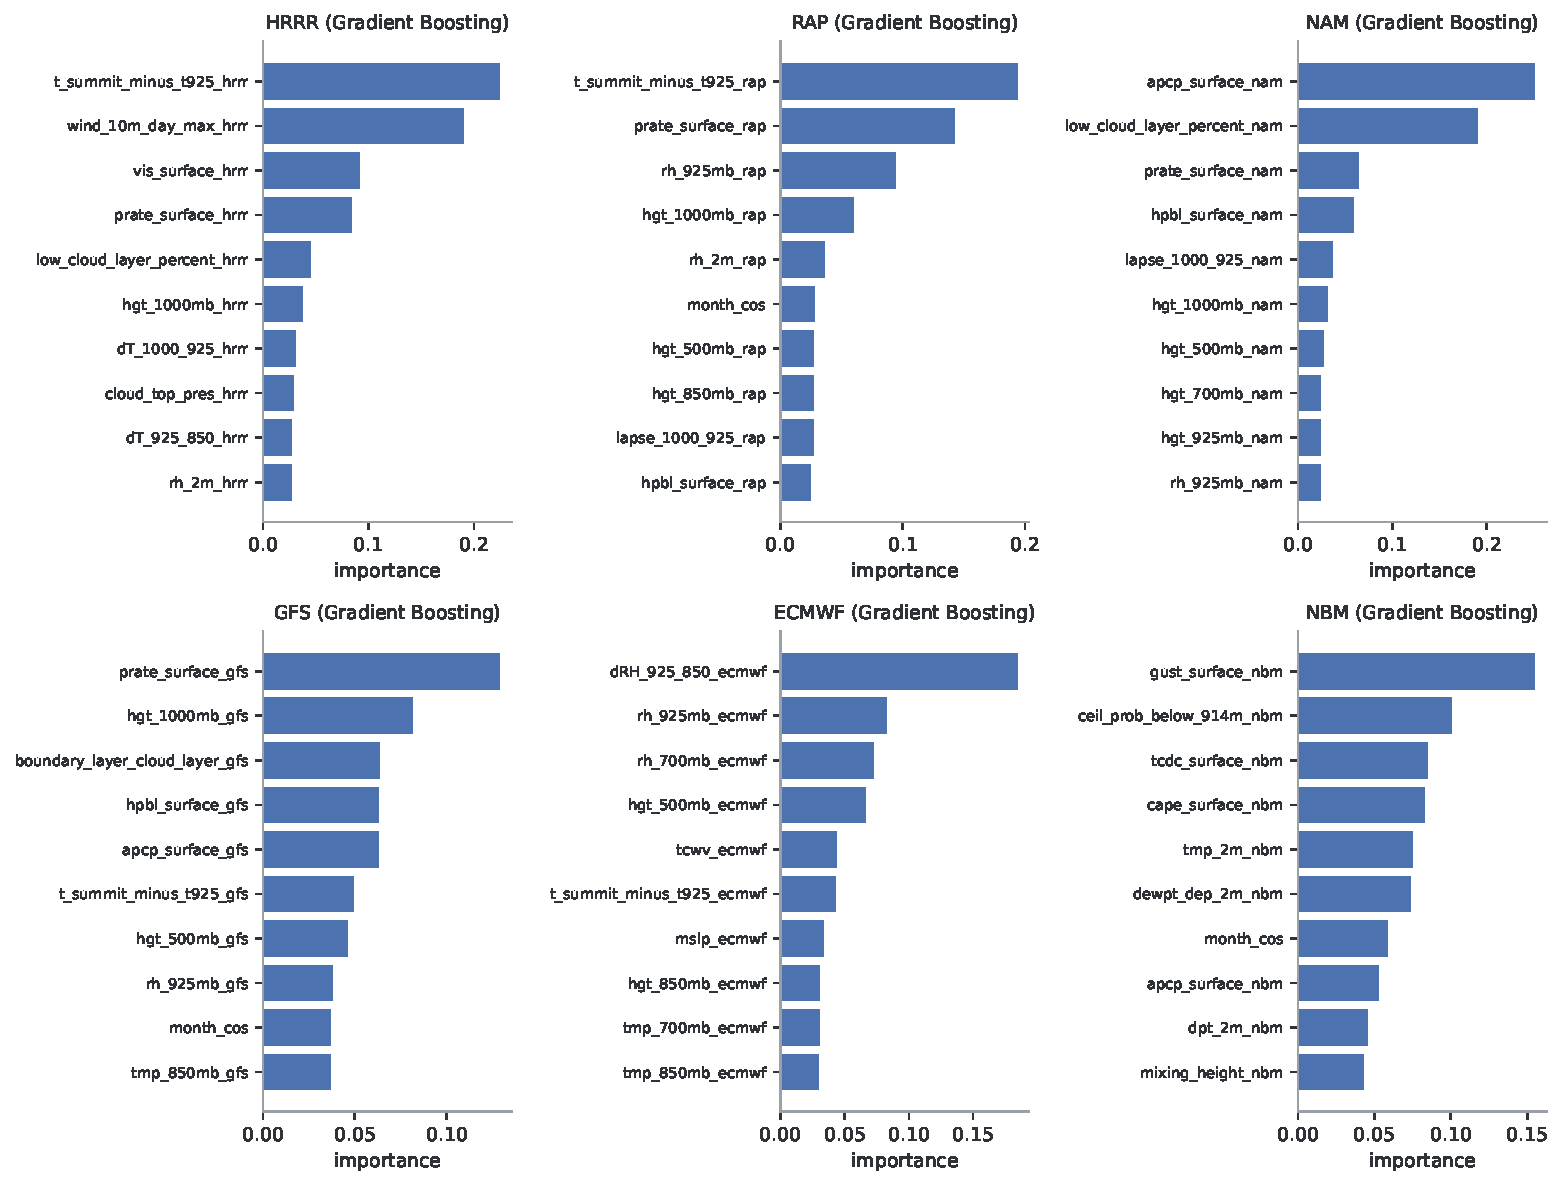
\includegraphics[width=\linewidth]{features_by_source.pdf}
\caption{Top 10 feature importances of each single-source Gradient Boosting model.}\label{fig:featsrc}
\end{figure}

\clearpage
%======================================================================
\section{Input parameters}\label{app:features}
%======================================================================
Each field is pulled from every NWP source that publishes it. Derived quantities are added: layer temperature differences and lapse rates
(\code{dT\_1000\_925}, \code{dT\_925\_850}, \code{dT\_850\_700}, \code{dT\_1000\_850}, \code{lapse\_*}),
\code{dRH\_925\_850}, the strongest inversion in the column (\code{max\_inversion}), summit-minus-level
temperatures (\code{t\_summit\_minus\_t925}, \code{t\_summit\_minus\_t1000}), and calendar encodings
(month and hour as sine/cosine).

\begin{table}[ht]\centering\small
\begin{tabularx}{\linewidth}{l Y}
\toprule
Key & Description\\
\midrule
\code{cloud\_top}, \code{cloud\_top\_hgt}, \code{cloud\_top\_pres} & Cloud-top height (AGL), geopotential height, pressure\\
\code{cloud\_base\_m}, \code{cloud\_base\_pres} & Cloud-base height (AGL) and pressure\\
\code{cloud\_ceiling\_m} & Height of the lowest BKN/OVC layer (AGL)\\
\code{low/middle/high\_cloud\_layer\_percent} & Cloud cover below $\sim$2\,km, 2--6\,km, above 6\,km\\
\code{tcdc\_surface}, \code{tcdc\_high\_cloud}, \code{cdcb\_high\_cloud} & Total and high cloud cover\\
\code{boundary\_layer\_cloud\_layer} & Cloud fraction within the planetary boundary layer\\
\code{tmp\_\{1000,925,850,700,500\}mb} & Temperature on pressure levels ($\sim$100, 750, 1500, 3000, 5500\,m)\\
\code{rh\_\{1000,925,850,700\}mb} & Relative humidity on pressure levels\\
\code{vvel\_\{925,850,700\}mb} & Vertical velocity on pressure levels\\
\code{hgt\_\{1000,925,850,700,500\}mb} & Geopotential height of pressure levels\\
\code{tmp\_2m}, \code{rh\_2m}, \code{dpt\_2m}, \code{dewpt\_dep\_2m} & Screen-level temperature, humidity, dewpoint and dewpoint depression\\
\code{t\_summit} & Temperature interpolated to the 1{,}917\,m summit\\
\code{hpbl\_surface}, \code{mixing\_height} & Planetary boundary-layer and mixing height\\
\code{cape}, \code{cape\_surface} & Convective available potential energy\\
\code{hgt\_0C\_iso} & Freezing level\\
\code{vis\_surface} & Surface visibility\\
\code{ceil\_prob\_below\_*}, \code{vis\_prob\_below\_*} & NBM probability of ceiling (152--2{,}012\,m) or visibility (1--5\,mi) below a threshold\\
\code{wind\_10m}, \code{wind\_10m\_day\_max}, \code{gust\_surface} & 10\,m wind, daily maximum, gust\\
\code{prate\_surface}, \code{apcp\_surface} & Precipitation rate and accumulation\\
\code{mslp}, \code{sp\_surface}, \code{tcwv} & Sea-level and surface pressure, column water vapour\\
\bottomrule
\end{tabularx}
\end{table}

\end{document}
